\documentclass[10pt,a5paper,openany]{report}
\usepackage{config}

\pagestyle{main}

%%%%%%%%%%%%%%%%%%%%%%%%%%%%%%%%%%%%%%%%%%%%%%%%%%%%%%%

\begin{document}

% ===== HALAMAN SAMPUL =====
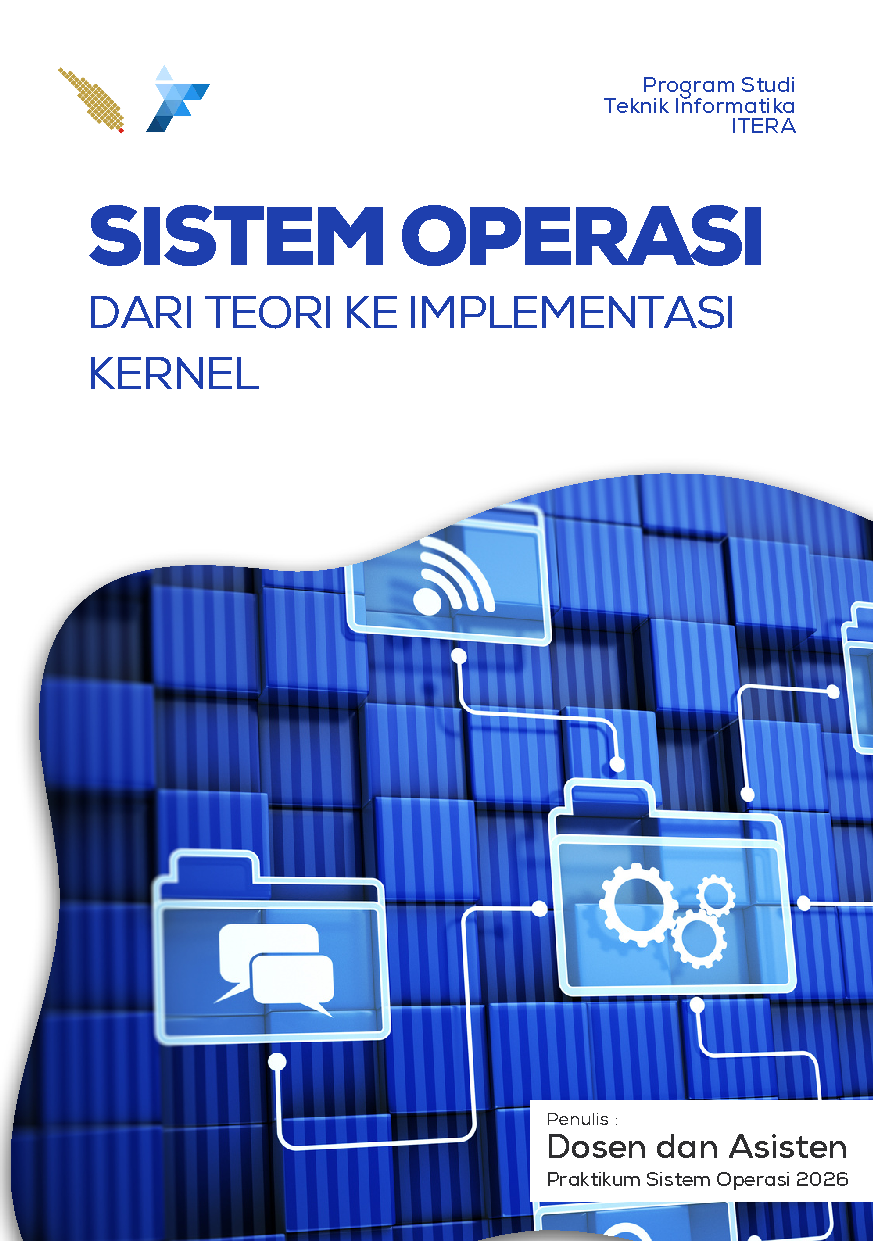
\includepdf[pages=1,noautoscale]{Figure/cover-front.pdf}

% ===== KATA PENGANTAR =====
\thispagestyle{empty}
\section*{Kata Pengantar}
Buku ini disusun dari materi \textit{Modul Praktikum} dan \textit{Hands-On} mata kuliah \courseName{} (\courseCode{}) di \institution{}. Setiap bab menggabungkan dasar teori, langkah-langkah praktikum, dan bagian \textbf{Latihan} berisi soal-soal untuk memperdalam pemahaman pembaca, disusun berurutan dari pengenalan konsep sistem operasi hingga implementasi komponen kernel (multi-threading, sinkronisasi, dan penjadwalan proses) pada sistem operasi \textit{bare-metal} 32-bit.
\newpage

% ===== DAFTAR ISI =====
\tableofcontents
\newpage

%%%%%%%%%%%%%%%%%%%%% BODY DOCUMENT %%%%%%%%%%%%%%%%%%%%%
\input{chapters/bab_01_pengenalan-os-vm}
% ============================================================
%  Modul 2 — Instalasi Ubuntu di VirtualBox
% ============================================================

\chapter{Instalasi Ubuntu di VirtualBox}
\label{chap:modul-02}

% --- 1. Tujuan dan Output Praktikum ---
\section{Tujuan dan Output Praktikum}

\subsection{Tujuan Praktikum}
Setelah menyelesaikan praktikum ini, mahasiswa diharapkan mampu:
\begin{enumerate}
    \item Menjelaskan langkah-langkah instalasi sistem operasi Ubuntu pada lingkungan VirtualBox.
    \item Mengonfigurasi mesin virtual sesuai dengan kebutuhan sistem (alokasi RAM, storage, dan CPU).
    \item Melakukan proses instalasi Ubuntu hingga sistem dapat dijalankan dengan baik sebagai Guest Operating System.
\end{enumerate}

\subsection{Output Praktikum}
Pada akhir praktikum ini, mahasiswa diharapkan menghasilkan:
\begin{itemize}
    \item Mesin virtual Ubuntu yang berhasil terinstal dan dapat dijalankan pada VirtualBox.
    \item Dokumentasi proses instalasi (screenshot tahapan penting instalasi).
    \item Laporan praktikum yang memuat konfigurasi mesin virtual serta hasil verifikasi sistem.
\end{itemize}


% --- 2. Dasar Teori ---
\newpage
\section{Dasar Teori}

\subsection{Konsep Virtualisasi dan Peran VirtualBox}
Virtualisasi adalah teknik untuk menjalankan sistem komputer virtual di atas komputer fisik yang sama. Pada praktikum ini, sistem operasi utama pada laptop atau PC Anda berperan sebagai \textit{host operating system}, sedangkan Ubuntu yang akan dipasang di dalam VirtualBox berperan sebagai \textit{guest operating system}. VirtualBox sendiri bertindak sebagai \textit{hypervisor type-2}, yaitu perangkat lunak yang meminjam sebagian sumber daya \textit{host} (CPU, RAM, penyimpanan, dan perangkat I/O) lalu menyajikannya sebagai mesin virtual mandiri bagi \textit{guest}.

Pendekatan ini penting dalam praktikum sistem operasi karena memberi lingkungan yang aman dan terisolasi. Kesalahan konfigurasi, eksperimen perintah, atau kegagalan \textit{boot} di dalam Ubuntu tidak langsung merusak sistem utama pengguna. Selain itu, seluruh mahasiswa dapat bekerja dengan lingkungan Linux yang relatif seragam meskipun komputer \textit{host}-nya berbeda-beda.

File \texttt{ISO} Ubuntu yang digunakan pada modul ini adalah citra media instalasi. Secara konseptual, berkas ini setara dengan keping DVD instalasi, hanya saja berbentuk file. Saat file ISO dipasangkan ke VM, firmware virtual akan melakukan \textit{boot} dari ISO tersebut dan memulai program instalasi Ubuntu.

\subsection{Komponen Konfigurasi Mesin Virtual}
Sebelum instalasi dimulai, VirtualBox meminta beberapa parameter konfigurasi. Masing-masing parameter memiliki fungsi teknis yang perlu dipahami agar pengaturan VM tidak dilakukan sekadar mengikuti klik antarmuka.

\begin{itemize}
    \item \textbf{Name}: penanda administrasi VM pada VirtualBox. Nama ini memudahkan identifikasi, tetapi tidak memengaruhi kinerja sistem.
    \item \textbf{ISO Image}: sumber media \textit{boot} awal yang berisi installer Ubuntu.
    \item \textbf{Username}, \textbf{Password}, dan \textbf{Hostname}: identitas akun awal dan nama mesin yang akan dipakai setelah instalasi selesai.
    \item \textbf{Base Memory (RAM)}: jumlah memori fisik \textit{host} yang dipinjam sementara oleh VM saat dijalankan. Jika terlalu kecil, installer dan sistem Ubuntu akan terasa lambat; jika terlalu besar, sistem \textit{host} dapat ikut kekurangan memori.
    \item \textbf{Processor}: jumlah inti CPU virtual yang dialokasikan. Menambah inti dapat mempercepat pekerjaan tertentu, tetapi alokasi berlebihan juga dapat membuat \textit{host} tidak responsif.
    \item \textbf{Virtual Hard Disk}: ruang penyimpanan virtual tempat Ubuntu, aplikasi, dan data \textit{guest} disimpan. Disk ini biasanya berupa file besar pada mesin \textit{host}.
\end{itemize}

Prinsip umumnya adalah membagi sumber daya secara seimbang. VM harus mendapat sumber daya yang cukup untuk berjalan lancar, tetapi sistem \textit{host} tetap harus menyisakan kapasitas agar VirtualBox dan aplikasi pendukung lain tetap stabil.

\subsection{Tahapan Umum Instalasi Ubuntu}
Secara umum, instalasi Ubuntu di VM berlangsung melalui empat tahap. Pertama, VM melakukan \textit{boot} dari file ISO dan menjalankan program installer. Kedua, installer menyalin berkas sistem dasar Ubuntu ke \textit{virtual hard disk}. Ketiga, installer membuat akun pengguna, nama komputer, dan konfigurasi awal lain. Keempat, sistem melakukan \textit{restart} dan \textit{boot} ulang dari disk virtual yang baru saja diisi, bukan lagi dari file ISO.

Memahami alur ini membantu mahasiswa membaca gejala saat instalasi berlangsung. Misalnya, jika VM gagal \textit{boot} dari awal, masalah biasanya berada pada pemilihan ISO atau urutan \textit{boot}. Jika proses sangat lambat, penyebab umumnya adalah alokasi RAM/CPU yang terlalu kecil. Jika setelah \textit{restart} sistem kembali ke installer, kemungkinan media \textit{boot} masih mengarah ke ISO, bukan ke disk virtual hasil instalasi.

Tabel \ref{tab:m02-dasar-teori} merangkum komponen inti yang perlu dipahami sebelum praktik instalasi.

\begin{table}[h]
\caption{Tabel Ringkasan Dasar Teori Modul 2}
\label{tab:m02-dasar-teori}
\centering
\begin{tabulary}{\textwidth}{|L|L|}
\hline
\textbf{Konsep} & \textbf{Penjelasan Singkat} \\ \hline
Host OS & Sistem operasi utama pada komputer fisik yang menjalankan VirtualBox. \\ \hline
Guest OS & Sistem operasi tamu (Ubuntu) yang dipasang dan dijalankan di dalam mesin virtual. \\ \hline
Hypervisor Type-2 & Perangkat lunak virtualisasi yang berjalan di atas \textit{host OS} untuk membuat dan mengelola VM. \\ \hline
ISO Image & Berkas citra instalasi yang digunakan VM sebagai media \textit{boot} awal. \\ \hline
Base Memory / Processor & Parameter alokasi sumber daya yang menentukan performa VM dan beban pada \textit{host}. \\ \hline
Virtual Hard Disk & Berkas penyimpanan virtual yang menjadi media instalasi dan data Ubuntu di dalam VM. \\ \hline
\end{tabulary}
\end{table}


% --- 3. Alat dan Bahan ---
\section{Alat dan Bahan}
\label{sec:alat-bahan}

\subsection{Perangkat Keras}
Untuk dapat menjalankan instalasi Ubuntu pada lingkungan virtual, diperlukan perangkat keras dengan spesifikasi minimum sebagai berikut:
\begin{itemize}
    \item Laptop atau PC dengan prosesor minimal dual-core.
    \item RAM minimal 4 GB (disarankan 8 GB untuk kinerja optimal).
    \item Ruang penyimpanan kosong minimal 25 GB.

\end{itemize}
Spesifikasi yang lebih tinggi akan meningkatkan performa mesin virtual selama proses instalasi dan penggunaan sistem.

\subsection{Perangkat Lunak}
Perangkat lunak yang diperlukan dalam praktikum ini meliputi:
\begin{itemize}
    \item Sistem Operasi utama (Windows, macOS, atau Linux) sebagai Host OS.
    \item Oracle VM VirtualBox 
    \item File ISO Ubuntu .
\end{itemize}
Pastikan VM VirtualBox dan file ISO Ubuntu telah diunduh sebelum praktikum dimuli untuk menghindari keterlambatan proses instalasi.

% --- 4. Langkah-Langkah Praktikum ---
\newpage
\section{Langkah-Langkah Praktikum}

\begin{enumerate}
    \item \textbf{Instalasi VirtualBox}

    Langkah pertama yang harus dilakukan adalah menginstal software virtualisasi, yaitu Oracle VM VirtualBox.

    Unduh VirtualBox melalui tautan resmi berikut:

    \url{https://www.virtualbox.org/wiki/Downloads}

    \item \textbf{Mengunduh File ISO Ubuntu Desktop}

    Setelah VirtualBox berhasil diinstal, langkah berikutnya adalah menyiapkan sistem operasi yang akan dijalankan di dalam Virtual Machine, yaitu Ubuntu Desktop.

    Unduh file ISO Ubuntu Desktop melalui tautan resmi berikut:

    \url{https://ubuntu.com/download/desktop}

    \item \textbf{Setup Virtual Machine}

    Setelah VirtualBox terinstal dan file ISO Ubuntu sudah diunduh, langkah selanjutnya adalah melakukan setup Virtual Machine di VirtualBox.

    \begin{enumerate}
        \item Buka aplikasi Oracle VM VirtualBox, kemudian klik tombol \textbf{New}.

        \begin{figure}[H]
            \centering
            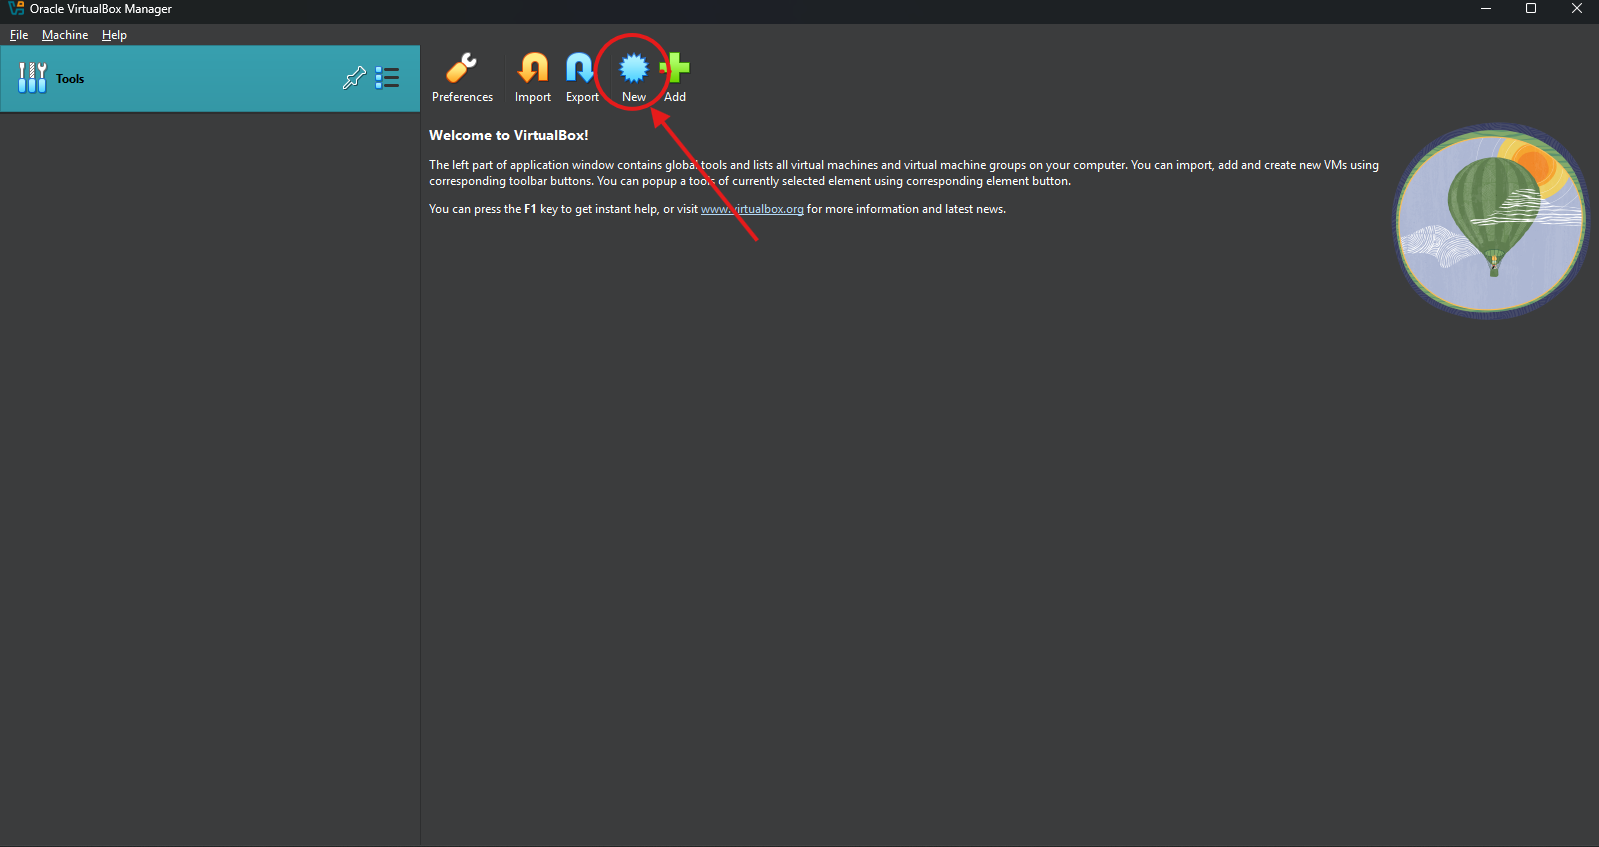
\includegraphics[width=0.75\textwidth]{Figure/02/gambar1.png}
            \caption{Tampilan Oracle VM VirtualBox saat memilih tombol \textbf{New}.}
            \label{fig:virtualbox-klik-new}
        \end{figure}
        \newpage
        \item Pada bagian \textbf{Name}, isi nama mesin virtual (misalnya \texttt{Ubuntu-Elsa}). Pada bagian \textbf{ISO Image}, pilih file ISO Ubuntu yang sudah diunduh, lalu klik \textbf{Next}. 

        \begin{figure}[H]
            \centering
            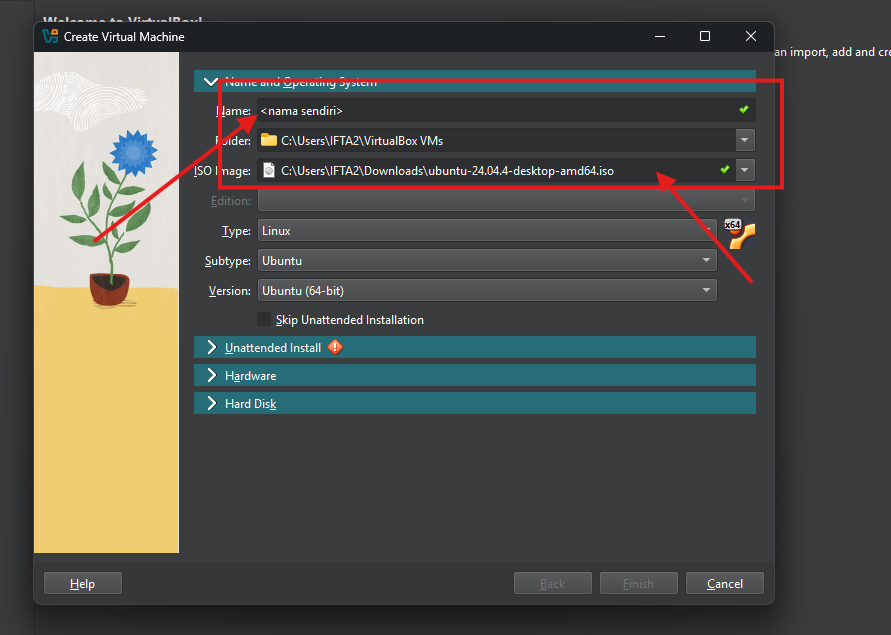
\includegraphics[width=0.75\textwidth]{Figure/02/gambar2.png}
            \caption{Tampilan Oracle VM VirtualBox saat memilih nama mesin virtual dan file ISO Ubuntu.}
            \label{fig:virtualbox-name-iso}
        \end{figure}

        \item Pada menu \textbf{Unattended Install}, isi \textbf{Username}, \textbf{Password}, dan \textbf{Hostname} (tanpa spasi), kemudian klik \textbf{Next}. 

        \begin{figure}[H]
            \centering
            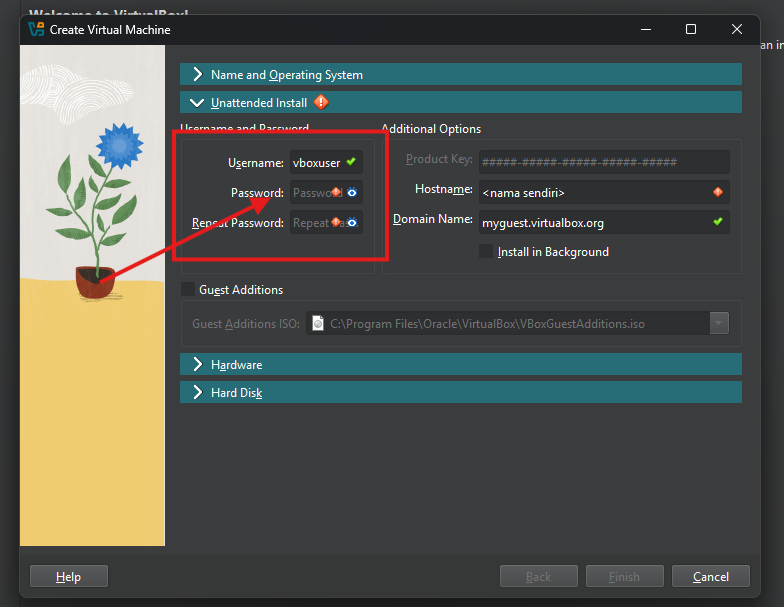
\includegraphics[width=0.75\textwidth]{Figure/02/gambar3.png}
            \caption{Tampilan Oracle VM VirtualBox pada tahap \textbf{Unattended Install}.}
            \label{fig:virtualbox-unattended-install}
        \end{figure}

        \item Pada menu \textbf{Hardware}, atur \textbf{Base Memory} minimal 4096 MB dan \textbf{Processor} minimal 2 core (sesuaikan dengan spesifikasi perangkat), lalu klik \textbf{Finish}. 

        \begin{figure}[H]
            \centering
            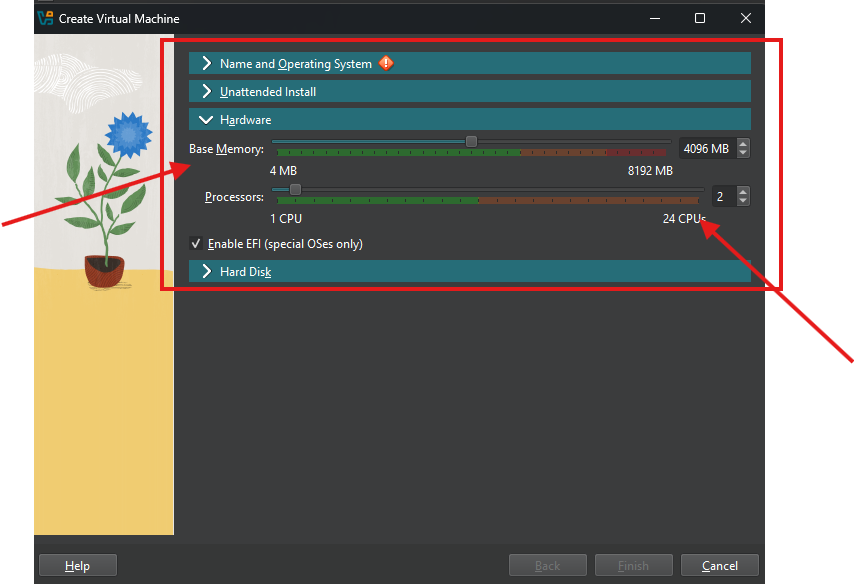
\includegraphics[width=0.75\textwidth]{Figure/02/gambar4.png}
            \caption{Tampilan pengaturan \textbf{Hardware} pada Oracle VM VirtualBox (Base Memory dan Processor).}
            \label{fig:virtualbox-hardware}
        \end{figure}

        \item Jalankan mesin virtual yang sudah dibuat, lalu pada tampilan awal instalasi pilih opsi \textbf{"Try or Install Ubuntu"}.

        \begin{figure}[H]
            \centering
            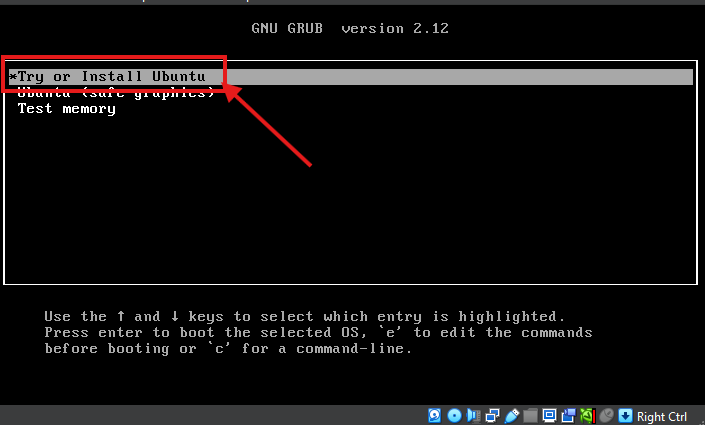
\includegraphics[width=0.75\textwidth]{Figure/02/gambar5.png}
            \caption{Tampilan awal instalasi Ubuntu saat memilih opsi \textbf{"Try or Install Ubuntu"}.}
            \label{fig:virtualbox-try-install}
        \end{figure}

        \item Lanjutkan proses instalasi sampai tahap \textit{copying files} selesai. Proses ini biasanya memerlukan waktu beberapa puluh menit, kemudian lakukan restart VM jika diminta. 
\end{enumerate}
\end{enumerate}

\newpage
\section{Latihan}

Pada bagian ini, setiap mahasiswa wajib mengerjakan tugas praktik mandiri sebagai berikut:
\begin{enumerate}
    \item Menginstal Ubuntu pada Oracle VM VirtualBox hingga sistem dapat berjalan dengan baik.
    \item Mendokumentasikan setiap langkah instalasi secara berurutan (wajib disertai bukti seperti tangkapan layar).
    \item Menyusun laporan praktikum sesuai template resmi pada GitHub IF ITERA:
    \url{https://github.com/informatika-itera/IF25-12007-Sistem-Operasi/tree/main/Hands-On}
\end{enumerate}

Laporan \textbf{wajib} disusun menggunakan \LaTeX.

\input{chapters/bab_03_navigasi-izin-linux}
\input{chapters/bab_04_bash-scripting}
\input{chapters/bab_07_booting-framework-os}
\input{chapters/bab_05_build-gcc}
\input{chapters/bab_06_makefile}
% ============================================================
%  Modul 8 — Implementasi Multi-threading
% ============================================================

\chapter{Implementasi Multi-threading}
\label{chap:modul-08}

% --- 1. Tujuan dan Output Praktikum ---
\section{Tujuan dan Output Praktikum}

\subsection{Tujuan Praktikum}
Tujuan yang diharapkan dapat dicapai oleh mahasiswa adalah:
\begin{enumerate}
	\item Memahami arsitektur perangkat lunak dalam manajemen \textit{thread} (termasuk abstraksi \textit{Thread Control Block}) dan algoritma penjadwalan (\textit{scheduling}) pada tingkat inti sistem operasi (\textit{kernel-level}).
	\item Mempraktikkan implementasi logika \textit{Context Switching} untuk memfasilitasi eksekusi \textit{multi-threading} melalui penyimpanan dan pemuatan status register CPU (memanfaatkan manipulasi bahasa tingkat rendah/Assembly).
\end{enumerate}

\subsection{Output Praktikum}
Hasil luaran yang diekspektasikan adalah kelengkapan instrumen berikut:
\begin{itemize}
	\item Implementasi fungsional dari modifikasi berkas sumber (khususnya penyesuaian pada logika \texttt{thread.c}, \texttt{switch.asm}, dan \texttt{scheduler.h}) yang terbukti mampu mengompilasi rekayasa antrean \textit{thread}.
	\item Tangkapan layar (\textit{screenshot}) keluaran terminal dari emulator QEMU yang memvalidasi bahwa beberapa \textit{thread} (contoh: Thread A, B, dan C) sukses berjalan saling bergantian secara sinkron mengambil alih siklus CPU.
\end{itemize}

% --- 2. Dasar Teori ---
\newpage
\section{Dasar Teori}

\subsection{Pengenalan Thread dan Multi-threading}
Dalam sistem komputasi, \textit{thread} adalah unit instruksi terkecil yang dapat dijadwalkan oleh sistem operasi \cite{Silberschatz2018}. Jika sebuah proses diibaratkan sebagai program yang sedang berjalan dan memiliki memori sendiri, maka \textit{thread} adalah entitas eksekusi operasional di dalam proses tersebut. Lingkungan OS \textit{bare-metal} merintis kerangka \textit{multi-threading} agar dapat mensimulasikan penanganan banyak fungsi bahasa C secara bersamaan (konkurensi) \cite{pintos_stanford}. Secara konseptual, rutinitas pembuatan dan pengelolaan \textit{thread} dikonstruksi guna mendistribusikan beban kerja secara seimbang sehingga mendongkrak efisiensi utilitas prosesor.

\subsection{Konteks Eksekusi dan Context Switching}
Konteks eksekusi merujuk pada seluruh status kumpulan register dari prosesor (seperti EAX, EBX, EBP, dan ESP pada perangkat arsitektur x86) yang dikenakan oleh sebuah \textit{thread} pada momentum waktu tertentu \cite{bryant2015computer}. Ketika sistem operasi hendak memberhentikan satu \textit{thread} lalu beralih ke giliran antrean eksekusi milik \textit{thread} yang lain, OS wajib menukarkan keadaannya lewat taktik perpindahan \textit{Context Switching}.

Karena kerumitan modifikasi letak tumpukan memori (\textit{stack}) amat bergantung pada wujud arsitektur silikon sistem biner, prosedur krusial ini umumnya direpresentasikan murni melalui arahan instruksi pada level \textit{Assembly}. Operasi tersebut mutlak ditugaskan untuk mengekstrak simpanan (\textit{Push}) dari *thread* lama seraya mengangkat muatan register (\textit{Pop}) profil milik antrean *thread* pengganti.

\subsection{Stack Awal \textit{Thread} Baru}
Sebuah \textit{thread} baru tidak muncul dalam keadaan "siap jalan" secara ajaib. Ketika \texttt{thread\_create()} dipanggil, kernel harus menyiapkan \textit{stack} awal sintetis yang isinya menyerupai hasil penyimpanan konteks normal. Dengan cara ini, saat \textit{scheduler} pertama kali memilih \textit{thread} tersebut, kode \textit{context switch} cukup melakukan \textit{restore register} dan melompat ke alamat yang sudah disusun sebelumnya.

Pada praktiknya, \textit{stack} awal ini biasanya memuat alamat fungsi masuk, parameter bantu, dan beberapa nilai register awal. Karena itulah modul ini mengarahkan mahasiswa menyusun beberapa \textit{frame} berlapis di memori. Tujuannya bukan sekadar memenuhi format struktur data, melainkan memastikan perpindahan pertama menuju \textit{thread} baru berlangsung melalui jalur yang sama seperti perpindahan konteks biasa.

\subsection{Siklus Hidup \textit{Thread} dan \textit{Ready Queue}}
Sepanjang hidupnya, sebuah \textit{thread} akan berpindah-pindah status. Setelah dibuat, \textit{thread} masuk ke status \textit{Ready}, yaitu siap dijadwalkan tetapi belum memegang CPU. Ketika dipilih oleh \textit{scheduler}, statusnya berubah menjadi \textit{Running}. Jika ia menyerahkan CPU secara sukarela melalui \texttt{yield()}, ia kembali ke antrean \textit{Ready}. Jika menunggu suatu kejadian atau sumber daya, statusnya menjadi \textit{Blocked}. Setelah pekerjaannya selesai, \textit{thread} akan keluar dari siklus ini.

\textit{Ready queue} adalah antrean \textit{thread} yang siap dieksekusi. TCB menyimpan identitas dan konteks tiap \textit{thread}, sedangkan \textit{ready queue} menyimpan urutan siapa yang berhak dipertimbangkan oleh \textit{scheduler}. Pemisahan konsep ini penting: TCB menjawab "siapa \textit{thread}-nya dan apa keadaannya", sedangkan antrean menjawab "siapa yang menunggu giliran CPU".

Pada modul ini, \textit{scheduler} yang dibangun masih bersifat sederhana. Ia belum memakai \textit{timer interrupt} untuk merebut CPU secara paksa. Artinya, perpindahan antar \textit{thread} sangat bergantung pada titik-titik sukarela seperti \texttt{yield()} atau blokade karena sinkronisasi.


\subsection{\textit{Cooperative Round-Robin} pada Modul Ini}
Algoritma penjadwalan yang dipakai sebagai fondasi modul ini adalah \textit{cooperative round-robin}. Istilah \textit{round-robin} berarti \textit{thread} yang siap dijalankan diputar bergiliran dari antrean \textit{ready}. Istilah \textit{cooperative} berarti perpindahan hanya terjadi ketika \textit{thread} yang sedang berjalan rela melepaskan CPU atau masuk ke kondisi \textit{blocked}; bukan karena dipotong paksa oleh \textit{timer interrupt}.

Kelebihan pendekatan ini adalah implementasinya lebih mudah dipahami untuk tahap awal, karena mahasiswa dapat memusatkan perhatian pada struktur antrean, penyimpanan konteks, dan alur \texttt{yield()}. Namun, model ini juga memiliki keterbatasan: jika satu \textit{thread} tidak pernah menyerahkan CPU, maka \textit{thread} lain dapat menunggu sangat lama. Keterbatasan inilah yang nantinya menjadi jembatan menuju pembahasan sinkronisasi dan penjadwalan yang lebih maju pada modul-modul berikutnya.

\subsection{Thread Control Block / TCB}
Agar sistem pengontrol sanggup menjaga identitas serta alokasi titik perhentian terakhir masing-masing \textit{thread}, direkayasa sebuah skema pelacak terstruktur dinamakan \textit{Thread Control Block} (TCB) \cite{Silberschatz2018}. Menggunakan struktur data mandiri (seperti halnya tipe rekaman mendasar pada bahasa C), blok TCB secara dedikatif membungkus parameter-parameter memori berikut:
\begin{itemize}
	\item \textbf{Thread ID}: Angka unit unik pengenal subyek yang tak boleh identik.
	\item \textbf{Status Thread}: Peta kondisi berjalannya instruksi pada suatu \textit{thread} (contoh: status sedang fasif siap diterjunkan/\textit{Ready}, status mandek/\textit{Blocked}, atau sedang berjalan/\textit{Running}).
	\item \textbf{Stack Pointer (ESP)}: Penunjuk referensi baris alamat terakhir yang terekam pada tumpukan (\textit{stack}) ketika interupsi perpindahan prosesnya berlangsung.
\end{itemize}

\subsection{Algoritma Penjadwalan (Scheduling)}
Siklus perancangan eksekusi CPU dikoordinasi secara tersentralisasi oleh modul OS benama \textit{Scheduler} \cite{Silberschatz2018}. Esensi utama dari algoritma komponen ini bertugas menyeleksi manakah prioritas \textit{thread} yang menduduki gerbang \textit{Ready} pada antrean sistem, agar mendapat wewenangnya dialihkan ke tingkatan fase \textit{Running}. Konsep paradigma fundamental penyeleksian dijabarkan melalui dua cara:
\begin{enumerate}
	\item \textbf{Cooperative Scheduling}: Sebuah \textit{thread} secara sadar membiarkan algoritma lain ganti mengeksekusi CPU dengan inisiatifnya menyerah (seperti metode inkuiri \texttt{yield()} atau tertahan menunggu sumber daya antarmuka selesai).
	\item \textbf{Preemptive Scheduling}: Sistem operasi menyetel batasan pencacah peranti keras layaknya \textit{Timer Interrupt}, berfungsi untuk merampas status dominasi algoritma tanpa ampun dari instruksi \textit{thread} yang sedang menduduki memori apakala batasan waktunya telah dirasa mencukupi.
\end{enumerate}

Tabel \ref{tab:m08-dasar-teori} memberikan intisari terminologi vital terkait landasan teori \textit{multithreading}.

\begin{table}[!ht]
	\caption{Tabel Ringkasan Dasar Teori Multi-threading}
	\label{tab:m08-dasar-teori}
	\centering
	\begin{tabulary}{\textwidth}{|L|L|}
		\hline
		\textbf{Konsep} & \textbf{Penjelasan Singkat} \\ \hline
		Thread & Unit eksekusi fungsional terkecil di dalam OS. \\ \hline
		Context Switch & Tindakan rekam-simpan silang arsitektur register satu \textit{thread} dengan \textit{thread} cadangan lainnya. \\ \hline
		TCB & Struktur blok tipe data spesifik pengingat status profil \textit{thread}. \\ \hline
		Scheduler & Organ algoritma OS yang mendikte hak pembagian waktu kendali CPU atas \textit{thread}. \\ \hline
	\end{tabulary}
\end{table}

% --- 3. Alat dan Bahan ---
\newpage
\section{Alat dan Bahan}
\label{sec:m08-alat-bahan}

\subsection{Perangkat Keras}
\begin{itemize}
	\item PC atau Laptop dengan arsitektur prosesor basis \textit{host} x86/x64 yang mendukung kelanjutan kompilasi emulator.
	\item Memori minimal 4GB RAM ruang eksekusi.
\end{itemize}

\subsection{Perangkat Lunak (Bahan Praktikum)}
\begin{itemize}
	\item OS \textit{Host} utama (Windows dengan WSL/GitBash, Linux, atau macOS).
	\item Text Editor (misalnya Visual Studio Code) untuk menyunting berkas kode bahasa C dan \textit{Assembly}.
	\item Instalasi Docker Engine (\texttt{docker.io}) untuk menyalakan lingkungan isolasi kompilasi.
	\item Emulator piranti keras x86: \texttt{qemu-system-x86} (atau instalasi QEMU setara) yang akan mengeksekusi binari hasil rakitan OS.
	\item Direktori \textit{Starter Code} OS 32-bit yang sudah disiapkan sebelumnya (berisi direktori \texttt{src} dengan kerangka lengkap \texttt{kernel.c}, \texttt{thread.h}, \texttt{thread.c}, \texttt{switch.asm}, \texttt{scheduler.h}, dsb).
\end{itemize}

% --- 4. Langkah-Langkah Praktikum ---
\newpage
\section{Langkah-Langkah Praktikum}

\subsection{Sesi 1: Persiapan Lingkungan Kerja}
\label{sec:m08-sesi-1}
Langkah pertama adalah menyiapkan direktori \textit{Starter Code} dan masuk ke dalam kontainer Docker.

\begin{enumerate}
	\item Buka terminal dan pastikan Anda berada di dalam folder \texttt{starter-code-os32-main}.
	\item Masuk ke lingkungan Docker dengan menjalankan perintah:
	      \begin{lstlisting}[language=bash, caption={Masuk ke lingkungan kontainer}]
./run-docker.sh
    \end{lstlisting}
	\item Buka berkas \texttt{src/thread.c} pada teks editor. Berkas ini adalah file utama yang akan dimodifikasi.
\end{enumerate}

\subsection{Sesi 2: Implementasi Fungsi \texttt{thread\_create()}}
\label{sec:m08-sesi-2}
Fungsi \texttt{thread\_create()} bertugas menyiapkan \textit{Thread Control Block} (TCB) dan \textit{stack} awal untuk \textit{thread} baru. Buka \texttt{thread.c}, cari fungsi pengisian \texttt{thread\_create}, dan ikuti langkah berikut:

\begin{enumerate}
	\item \textbf{Langkah 1 (Alokasi TCB):} Gunakan \texttt{allocate\_thread\_page()} untuk alokasi memori \textit{thread}. Jika berhasil, panggil \texttt{init\_thread(t, name, priority)} dan berikan ID dengan \texttt{t->tid = allocate\_tid()}.
	      \begin{figure}[H]
		      \centering
		      
\includegraphics[width=0.8\textwidth]{Figure/08/1.png}
		      \caption{Implementasi Alokasi TCB pada fungsi thread\_create()}
	      \end{figure}

	\item \textbf{Langkah 2 (Frame 1: \texttt{kernel\_thread\_frame}):} Buat variabel \textit{frame} ini menggunakan \texttt{alloc\_frame()}. Isi \texttt{eip} dengan \texttt{NULL}, lalu isi \texttt{function} dan \texttt{aux} sesuai dengan argumen parameter yang dikirim.
	      \begin{figure}[H]
		      \centering
		      
\includegraphics[width=0.8\textwidth]{Figure/08/2.png}
		      \caption{Implementasi Frame 1 pada fungsi thread\_create()}
	      \end{figure}

	\item \textbf{Langkah 3 (Frame 2: \texttt{switch\_entry\_frame}):} Buat variabel \textit{frame} ini dengan alokasi di bawah Frame 1. Isi \texttt{eip} dengan memanggil alamat fungsi \texttt{kernel\_thread}.
	      \begin{figure}[H]
		      \centering
		      
\includegraphics[width=0.8\textwidth]{Figure/08/3.png}
		      \caption{Implementasi Frame 2 pada fungsi thread\_create()}
	      \end{figure}

	\item \textbf{Langkah 4 (Frame 3: \texttt{switch\_threads\_frame}):} Buat variabel \textit{frame} terbawah ini. Isi variabel \texttt{eip} dengan \texttt{switch\_entry}, lalu set nilai \texttt{ebp}, \texttt{ebx}, \texttt{esi}, dan \texttt{edi} menjadi \texttt{0}.
	      \begin{figure}[H]
		      \centering
		      
\includegraphics[width=0.8\textwidth]{Figure/08/4.png}
		      \caption{Implementasi Frame 3 pada fungsi thread\_create()}
	      \end{figure}

	\item \textbf{Langkah 5 (Penyelesaian):} Panggil \texttt{thread\_unblock(t)} agar dimasukkan ke dalam antrean \textit{ready}, kemudian lakukan \textit{return} id \textit{thread} tersebut (\texttt{t->tid}).
	      \begin{figure}[H]
		      \centering
		      
\includegraphics[width=0.8\textwidth]{Figure/08/5.png}
		      \caption{Langkah Penyelesaian pada fungsi thread\_create()}
	      \end{figure}

	\item Pastikan kerangka utuh fungsi Anda menyerupai format referensi ini:
	      \begin{figure}[H]
		      \centering
		      
\includegraphics[width=0.8\textwidth]{Figure/08/6.png}
		      \caption{Fungsi utuh \texttt{thread\_create()} secara keseluruhan}
	      \end{figure}
\end{enumerate}

\subsection{Sesi 3: Implementasi Cooperative \textit{Round-Robin}}
\label{sec:m08-sesi-3}
Bagian ini mengatur agar \textit{thread} dapat saling bergantian menggunakan wewenang CPU. Masih di dalam file \texttt{thread.c}:

\begin{enumerate}
	\item \textbf{Modifikasi \texttt{thread\_yield()}:} Ambil \textit{thread} yang saat ini berjalan menggunakan \texttt{thread\_current()}. Ubah statusnya menjadi \texttt{THREAD\_READY}. Masukkan \textit{thread} ini ke dalam antrean \texttt{ready\_queue} pada indeks \texttt{ready\_tail}. Geser urutan \texttt{ready\_tail}, tambahkan jumlah \texttt{ready\_count}, dan akhiri dengan memanggil fungsi \texttt{schedule()}.
	      \begin{figure}[H]
		      \centering
		      
\includegraphics[width=0.8\textwidth]{Figure/08/7.png}
		      \caption{Implementasi fungsi \texttt{thread\_yield()}}
	      \end{figure}

	\item \textbf{Modifikasi \texttt{next\_thread\_to\_run()}:} Fungsi ini berjalan secara metode FIFO (\textit{First-In-First-Out}). Jika antrean kosong (\texttt{ready\_count} bernilai 0), kembalikan \texttt{initial\_thread}. Jika isi antrean tersedia, ambil \textit{thread} dari urutan depan (\texttt{ready\_queue[ready\_head]}), geser letak indeks depan \texttt{ready\_head}, kurangi nilai hitung \texttt{ready\_count}, lalu \textit{return thread} yang diambil tersebut.
	      \begin{figure}[H]
		      \centering
		      
\includegraphics[width=0.8\textwidth]{Figure/08/8.png}
		      \caption{Implementasi fungsi \texttt{next\_thread\_to\_run()}}
	      \end{figure}
\end{enumerate}

\subsection{Sesi 4: Kompilasi dan Pengujian QEMU}
\label{sec:m08-sesi-4}
Setelah seluruh kode di \texttt{thread.c} selesai, jalankan pengujian sistem untuk membuktikan bahwa OS sudah sanggup menjalankan perpindahan waktu \textit{thread}.

\begin{enumerate}
	\item Buka kembali terminal yang berada di dalam lingkungan Docker, lalu jalankan perintah kompilasi:
	      \begin{lstlisting}[language=bash, caption={Perintah build pada terminal Docker}]
make
    \end{lstlisting}
	\item Setelah proses kompilasi selesai (\textit{error} tidak muncul), jalankan QEMU emulator secara langsung menggunakan perintah di bawah ini:
	      \begin{lstlisting}[language=bash, caption={Menjalankan OS pada terminal Docker}]
make run
    \end{lstlisting}
	\item Perhatikan layar simulator QEMU. Anda harus masuk dalam putaran sistem \textit{infinite loop} yang memperlihatkan ketiga \textit{thread} yang dibuat mencetak teks (Thread A, Thread B, dan Thread C) bergantian per waktu putaran:
	      \begin{lstlisting}[caption={Ekspektasi output sistem penjadwalan Thread di latar QEMU}]
===================================
  IF-OS  |  Praktikum Sistem Operasi
===================================

Inisialisasi sistem thread...
Membuat thread A, B, C...
Memulai scheduling...

[Thread A] tick 0
[Thread B] tick 0
[Thread C] tick 0
[Thread A] tick 1
[Thread B] tick 1
...
    \end{lstlisting}
\end{enumerate}

% ----------------------------------------------------------------
\section{Latihan}

% ----------------------------------------------------------------
\subsection{Tujuan}

Jawablah pertanyaan-pertanyaan berikut berdasarkan hasil praktikum Anda
sesuai urutan sesi pada Modul~8.
Sertakan bukti berupa \textit{screenshot} atau penggalan keluaran
terminal yang relevan pada setiap jawaban.

% ----------------------------------------------------------------
\subsection{Sesi 1: Persiapan Lingkungan Kerja}

\subsubsection{Masuk ke Container Docker}

Jalankan perintah berikut di terminal, kemudian masuk ke direktori
\textit{workspace}:

\begin{lstlisting}[language=bash, caption={Menjalankan container dan masuk workspace}]
docker run --rm -it \
    -v "C:\path\ke\starter-code:/workspace" \
    sinanonym/ifos-env
cd /workspace
\end{lstlisting}

\begin{enumerate}

	\item \textbf{Compile starter code sebelum implementasi.}\\
	      Jalankan perintah berikut di dalam container:

	      \begin{lstlisting}[language=bash, caption={Perintah kompilasi awal}]
make clean && make
    \end{lstlisting}

	      Tuliskan seluruh \textit{warning} yang muncul pada saat kompilasi dan
	      jelaskan mengapa \textit{warning} tersebut muncul pada kode
	      \textit{stub}.

	\item \textbf{Jalankan QEMU sebelum implementasi.}\\
	      Jalankan perintah berikut lalu sertakan \textit{screenshot} layar QEMU.
	      Jelaskan mengapa sistem berhenti di sana dan belum menampilkan
	      output Thread~A/B/C.

	      \begin{lstlisting}[language=bash, caption={Menjalankan emulator QEMU}]
make run
    \end{lstlisting}


\end{enumerate}

% ----------------------------------------------------------------
\subsection{Sesi 2: Implementasi \texttt{thread\_create()}}

\subsubsection{Thread Control Block dan Layout Memori}

\begin{enumerate}

	\item \textbf{Field-field \texttt{struct thread}.}\\
	      Perhatikan definisi \texttt{struct thread} di \texttt{src/thread.h}.
	      Isilah tabel berikut berdasarkan kode sumber.

	      \begin{table}[!ht]
		      \caption{Field-field pada \texttt{struct thread}}
		      \label{tab:h04-struct-thread}
		      \centering
		      \begin{tabulary}{\linewidth}{|L|L|L|}
			      \hline
			      \textbf{Field} & \textbf{Tipe Data} & \textbf{Fungsi} \\
			      \hline
			      \texttt{tid}      & \texttt{tid\_t}              & \textit{[Isi]} \\
			      \hline
			      \texttt{status}   & \texttt{enum thread\_status} & \textit{[Isi]} \\
			      \hline
			      \texttt{name}     & \texttt{char[16]}            & \textit{[Isi]} \\
			      \hline
			      \texttt{stack}    & \texttt{uint8\_t *}          & \textit{[Isi]} \\
			      \hline
			      \texttt{priority} & \texttt{int}                 & \textit{[Isi]} \\
			      \hline
			      \texttt{magic}    & \texttt{unsigned}            & \textit{[Isi]} \\
			      \hline
		      \end{tabulary}
	      \end{table}

	\item \textbf{Layout halaman 4~KB setiap thread.}\\
	      Setiap thread menempati satu halaman (\textit{page}) memori berukuran
	      4~KB. Isilah kolom \textit{Isi} pada tabel layout di bawah ini
	      untuk menggambarkan posisi \texttt{struct thread}, \textit{stack},
	      dan ketiga frame yang disiapkan oleh \texttt{thread\_create()}.

	      \begin{table}[!ht]
		      \caption{Layout halaman 4~KB milik sebuah thread}
		      \label{tab:h04-page-layout}
		      \centering
		      \begin{tabulary}{\linewidth}{|C|L|}
			      \hline
			      \textbf{Offset (relatif)} & \textbf{Isi} \\
			      \hline
			      \texttt{+4096} & \textit{[Isi: puncak halaman / ESP awal]} \\
			      \hline
			      \texttt{...}   & \texttt{switch\_threads\_frame} \\
			      \hline
			      \texttt{...}   & \texttt{switch\_entry\_frame} \\
			      \hline
			      \texttt{...}   & \texttt{kernel\_thread\_frame} \\
			      \hline
			      \texttt{...}   & \textit{[Isi: area stack kosong, tumbuh ke bawah ($\downarrow$)]} \\
			      \hline
			      \texttt{+0}    & \texttt{struct thread} (TCB) \\
			      \hline
		      \end{tabulary}
	      \end{table}

	\item \textbf{Analisis fungsi \texttt{running\_thread()}.}\\
	      Perhatikan potongan kode berikut:

	      \begin{lstlisting}[language=c, caption={Implementasi \texttt{running\_thread()} di \texttt{src/thread.c}}]
struct thread *running_thread(void) {
    uint32_t esp;
    __asm__ volatile ("mov %%esp, %0" : "=g" (esp));
    return (struct thread *)(void *)(esp & ~(uint32_t)(PGSIZE - 1));
}
    \end{lstlisting}

	      \begin{enumerate}
		      \item[(a)] Jelaskan apa yang dilakukan operasi bitwise
		            \texttt{esp \& \textasciitilde(PGSIZE - 1)} dan
		            mengapa hasilnya selalu merupakan alamat awal
		            \textit{page}.

		      \item[(b)] Mengapa teknik ini hanya benar jika
		            \texttt{struct thread} selalu berada di offset~0
		            dari halamannya? Apa dampaknya jika
		            \texttt{initial\_thread\_page} di \texttt{boot.asm}
		            tidak di-\textit{align} ke 4096~byte?

		      \item[(c)] Apa fungsi \texttt{THREAD\_MAGIC} dan bagaimana
		            \texttt{thread\_current()} menggunakannya untuk
		            mendeteksi \textit{stack overflow}?
	      \end{enumerate}

\end{enumerate}

\subsubsection{Implementasi Fungsi \texttt{thread\_create()}}

\begin{enumerate}

	\item \textbf{Tiga stack frame pada \texttt{thread\_create()}.}\\
	      Isilah tabel berikut berdasarkan komentar petunjuk di
	      \texttt{src/thread.c}.

	      \begin{table}[!ht]
		      \caption{Tiga stack frame yang disiapkan \texttt{thread\_create()}}
		      \label{tab:h04-stack-frames}
		      \centering
		      \begin{tabulary}{\linewidth}{|C|L|L|L|}
			      \hline
			      \textbf{Urutan push} & \textbf{Nama frame} &
			      \textbf{Field penting} & \textbf{Nilai yang diisi} \\
			      \hline
			      1, paling atas & \texttt{kernel\_\allowbreak thread\_\allowbreak frame} &
			      \texttt{eip}, \texttt{function}, \texttt{aux} &
			      \textit{[Isi]} \\
			      \hline
			      2, tengah & \texttt{switch\_\allowbreak entry\_\allowbreak frame} &
			      \texttt{eip} &
			      \textit{[Isi]} \\
			      \hline
			      3, paling bawah & \texttt{switch\_\allowbreak threads\_\allowbreak frame} &
			      \texttt{eip}, register \textit{callee-saved} &
			      \textit{[Isi]} \\
			      \hline
		      \end{tabulary}
	      \end{table}

	\item \textbf{Alur eksekusi pertama thread baru.}\\
	      Saat thread baru \textbf{pertama kali} dijadwalkan melalui
	      \texttt{switch\_threads()}, jelaskan secara berurutan apa yang
	      terjadi mulai dari \texttt{switch\_entry} hingga fungsi thread
	      (\texttt{func\_a}, \texttt{func\_b}, atau \texttt{func\_c})
	      benar-benar mulai berjalan.

	\item \textbf{Tulis implementasi \texttt{thread\_create()}.}\\
	      Salin kode yang telah Anda tulis di \texttt{src/thread.c}:

	      \begin{lstlisting}[language=c, caption={Implementasi \texttt{thread\_create()} oleh mahasiswa}]
tid_t thread_create(const char *name, int priority,
                    thread_func *function, void *aux) {

    /* Tulis implementasi Anda di sini */

}
    \end{lstlisting}

	\item \textbf{Penanganan kegagalan alokasi.}\\
	      Kapan \texttt{allocate\_thread\_page()} dapat mengembalikan
	      \texttt{NULL}, dan bagaimana \texttt{thread\_create()} harus
	      menanganinya?

\end{enumerate}

% ----------------------------------------------------------------
\subsection{Sesi 3: Implementasi \textit{Cooperative Round-Robin}}

\subsubsection{Konsep Status Thread}

\begin{enumerate}

	\item \textbf{Perbedaan \texttt{THREAD\_READY} dan
		      \texttt{THREAD\_BLOCKED}.}\\
	      Lengkapi tabel perbandingan berikut.

	      \begin{table}[!ht]
		      \caption{Perbandingan status \texttt{THREAD\_READY} dan \texttt{THREAD\_BLOCKED}}
		      \label{tab:h04-thread-status}
		      \small
		      \begin{tabularx}{\linewidth}{|X|X|X|}
			      \hline
			      \textbf{Aspek} &
			      \makecell[l]{\textbf{THREAD\_}\\\textbf{READY}} &
			      \makecell[l]{\textbf{THREAD\_}\\\textbf{BLOCKED}} \\
			      \hline
			      Siapa yang menetapkan? & \textit{[Isi]} & \textit{[Isi]} \\
			      \hline
			      Masuk ke \textit{ready queue}? & \textit{[Isi]} & \textit{[Isi]} \\
			      \hline
			      Cara kembali ke \texttt{RUNNING} & \textit{[Isi]} & \textit{[Isi]} \\
			      \hline
			      Contoh penggunaan & \textit{[Isi]} & \textit{[Isi]} \\
			      \hline
		      \end{tabularx}
	      \end{table}

\end{enumerate}

\subsubsection{Implementasi Fungsi \textit{Scheduling}}

\begin{enumerate}

	\item \textbf{Tulis implementasi \texttt{thread\_yield()}.}\\
	      Salin kode yang telah Anda tulis di \texttt{src/thread.c}:

	      \begin{lstlisting}[language=c, caption={Implementasi \texttt{thread\_yield()} oleh mahasiswa}]
void thread_yield(void) {

    /* Tulis implementasi Anda di sini */

}
    \end{lstlisting}

	\item \textbf{Tulis implementasi \texttt{next\_thread\_to\_run()}
		      (Round-Robin FIFO).}\\
	      Salin kode yang telah Anda tulis di \texttt{src/thread.c}:

	      \begin{lstlisting}[language=c, caption={Implementasi \texttt{next\_thread\_to\_run()} oleh mahasiswa}]
struct thread *next_thread_to_run(void) {

    /* Tulis implementasi Anda di sini */

}
    \end{lstlisting}

	\item \textbf{Mengapa mengembalikan \texttt{initial\_thread},
		      bukan \texttt{NULL}?}\\
	      Jelaskan apa yang akan terjadi pada fungsi \texttt{schedule()} jika
	      \texttt{next\_thread\_to\_run()} mengembalikan \texttt{NULL} saat
	      antrian kosong.

	\item \textbf{\texttt{thread\_block()} vs.\ \texttt{thread\_yield()}
		      di akhir \texttt{kernel\_main}.}\\
	      Jelaskan perbedaan perilaku kedua fungsi tersebut setelah Thread~A,
	      B, dan C berhasil dibuat, dan mengapa \texttt{thread\_block()}
	      adalah pilihan yang benar.

\end{enumerate}

% ----------------------------------------------------------------
\subsection{Sesi 4: Kompilasi dan Pengujian QEMU}

\begin{enumerate}

	\item \textbf{Compile ulang setelah implementasi selesai.}

	      \begin{lstlisting}[language=bash, caption={Perintah build dan run setelah implementasi}]
make clean && make && make run
    \end{lstlisting}

	      Sertakan \textit{screenshot} layar QEMU yang menampilkan ketiga
	      thread berjalan bergantian.


	\item \textbf{Verifikasi urutan penjadwalan.}\\
	      Ekspektasi keluaran sistem yang benar adalah sebagai berikut:

	      \begin{lstlisting}[caption={Ekspektasi output Round-Robin di layar QEMU}]
===================================
  IF-OS  |  Praktikum Sistem Operasi
===================================

Inisialisasi sistem thread...
Membuat thread A, B, C...
Memulai scheduling...

[Thread A] tick 0
[Thread B] tick 0
[Thread C] tick 0
[Thread A] tick 1
[Thread B] tick 1
[Thread C] tick 1
...
    \end{lstlisting}

	      Apakah urutan Thread~A $\to$ Thread~B $\to$ Thread~C $\to$
	      Thread~A $\to \ldots$ terjaga secara konsisten pada hasil Anda?
	      Jelaskan mengapa urutan ini dapat dijamin oleh implementasi FIFO
	      pada \textit{ready queue}.

	\item \textbf{Analisis \textit{warning} compiler sebelum dan setelah
		      implementasi.}\\
	      Apakah \textit{warning} \texttt{unused-function} dan
	      \texttt{unused-variable} yang muncul sebelum implementasi masih
	      ada setelah Anda mengimplementasikan ketiga fungsi? Jelaskan
	      mengapa \textit{warning} tersebut hilang.

\end{enumerate}

% ----------------------------------------------------------------
\subsection{Eksplorasi Mandiri}

\begin{enumerate}

	\item \textbf{Menambah Thread keempat.}\\
	      Tambahkan Thread~D dengan fungsi dan warna VGA berbeda di
	      \texttt{src/kernel.c}, kemudian compile ulang dan jalankan.

	      \begin{enumerate}
		      \item[(a)] Sertakan \textit{screenshot} layar QEMU yang
		            menampilkan empat thread berjalan bergantian.


		      \item[(b)] Berapa nilai \texttt{MAX\_THREADS} saat ini?
		            Apa yang terjadi jika Anda membuat thread melebihi
		            batas tersebut? Tunjukkan dengan percobaan dan
		            sertakan bukti.
	      \end{enumerate}

	\item \textbf{Simulasi \textit{finite thread}.}\\
	      Ubah \texttt{func\_a} di \texttt{src/kernel.c} agar hanya
	      mencetak \textbf{5 kali} lalu berhenti (ganti \texttt{while(1)}
	      dengan loop terbatas). Amati apakah Thread~B dan Thread~C tetap
	      berjalan setelah Thread~A selesai, lalu jelaskan peran
	      \texttt{thread\_exit()} dalam skenario ini.

	\item \textbf{Refleksi: \textit{cooperative} vs.\
		      \textit{preemptive scheduling}.}\\
	      Sistem IF-OS saat ini menggunakan \textit{cooperative scheduling}
	      di mana thread hanya berganti saat secara sadar memanggil
	      \texttt{thread\_yield()}.

	      \begin{enumerate}
		      \item[(a)] Apa kelemahan utama \textit{cooperative scheduling}
		            dibandingkan \textit{preemptive scheduling}?
		            Berikan contoh skenario nyata di mana kelemahan
		            ini berbahaya.

		      \item[(b)] Komponen perangkat keras apa yang perlu ditambahkan
		            agar kernel dapat memaksa pergantian thread secara
		            otomatis tanpa bergantung pada kepatuhan thread
		            itu sendiri?
	      \end{enumerate}

\end{enumerate}

\input{chapters/bab_09_race-condition}
% ============================================================
%  Modul 10 — Implementasi Mutex dan Locks
% ============================================================

\chapter{Implementasi Mutex dan Locks}
\label{chap:modul-10}

% --- 1. Tujuan dan Output Praktikum ---
\section{Tujuan dan Output Praktikum}

\subsection{Tujuan Praktikum}
Setelah menyelesaikan praktikum ini, mahasiswa diharapkan mampu:
\begin{enumerate}
	\item Memahami cara kerja \textit{semaphore} sebagai mekanisme dasar sinkronisasi antar \textit{thread}.
	\item Memahami konsep \textit{mutex} (\textit{Mutual Exclusion Lock}) dan perbedaannya dengan \textit{semaphore} secara semantik maupun struktural.
	\item Mengimplementasikan mekanisme penahanan (\textit{wait}) dan pelepasan (\textit{signal}) sumber daya, serta sistem penguncian eksklusif pada tingkat kernel.
	\item Memverifikasi efektivitas mekanisme sinkronisasi yang dibangun dalam mencegah dan menghilangkan \textit{race condition} yang diamati pada modul sebelumnya.
\end{enumerate}

\subsection{Output Praktikum}
Pada akhir praktikum ini, mahasiswa diharapkan menghasilkan:
\begin{itemize}
	\item Implementasi algoritma sinkronisasi kernel yang valid dan mampu meregulasi antrean \textit{thread} dengan tepat.
	\item Simulasi sistem operasi yang mendemonstrasikan penyelesaian skenario \textit{Producer-Consumer} dengan eksekusi yang tersinkronisasi, rapi, dan konsisten.
	\item Laporan analisis yang menjabarkan bagaimana struktur \textit{semaphore} dan \textit{lock} bekerja sama secara harmonis untuk melindungi area \textit{critical section} dari interupsi paksa.
\end{itemize}

% --- 2. Dasar Teori ---
\newpage
\section{Dasar Teori}

\subsection{Konsep Semaphore}

\textit{Semaphore} adalah sebuah struktur data abstrak yang digunakan untuk mengoordinasikan akses beberapa \textit{thread} atau proses terhadap sumber daya (\textit{shared resource}) yang jumlahnya terbatas.
Konsep ini pertama kali diperkenalkan oleh ilmuwan komputer Edsger W. Dijkstra pada tahun 1965.

Secara konseptual, \textit{semaphore} bekerja seperti "keranjang berisi token". Jika sebuah \textit{thread} ingin melakukan pekerjaan, ia harus mengambil satu token dari keranjang. Jika keranjang kosong,
\textit{thread} tersebut harus menunggu (mengantre) sampai ada token yang dikembalikan oleh \textit{thread} lain.

Di dalam sistem operasi, sebuah \textit{semaphore} terdiri dari dua komponen utama:
\begin{enumerate}
	\item Sebuah variabel bilangan bulat (integer) non-negatif yang mewakili "jumlah token" atau kapasitas sumber daya.
	\item Sebuah antrean (\textit{waiting queue}) untuk menampung \textit{thread} yang sedang menunggu giliran.
\end{enumerate}

Semaphore dikendalikan melalui dua operasi atomik (tidak dapat diinterupsi):
\begin{itemize}
	\item \textbf{Operasi \texttt{Wait(S)} (P atau \textit{Proberen})}: Mengurangi nilai variabel semaphore. Jika nilainya menjadi $0$ (atau kurang), maka \textit{thread} yang mengeksekusi operasi ini akan diubah
	      statusnya menjadi \textit{Blocked} / \textit{Asleep} dan dimasukkan ke dalam antrean. Pada sistem OS, operasi ini dinamakan \texttt{sema\_down()}.
	\item \textbf{Operasi \texttt{Signal(S)} (V atau \textit{Verhogen})}: Menambah nilai variabel semaphore. Jika ada \textit{thread} yang sedang mengantre (tertidur), operasi ini akan membangunkan (\textit{Wake up})
	      salah satu \textit{thread} tersebut agar siap dieksekusi kembali oleh CPU. Pada sistem OS, operasi ini dinamakan \texttt{sema\_up()}.
\end{itemize}

Berdasarkan kapasitasnya, semaphore dibagi menjadi dua:
\begin{enumerate}
	\item \textbf{Counting Semaphore}: Nilainya bisa berapa saja ($\geq 0$). Sangat berguna untuk mengontrol akses ke *resource* yang memiliki batasan jumlah, seperti jumlah tempat parkir kosong, atau sisa kapasitas \textit{buffer}.
	\item \textbf{Binary Semaphore}: Nilainya hanya dibatasi pada angka $0$ dan $1$. Sering digunakan untuk menjamin \textit{Mutual Exclusion}.
\end{enumerate}

\subsection{Atomisitas Operasi Sinkronisasi}
Meskipun \textit{semaphore} terlihat seperti bilangan pencacah biasa, operasi \texttt{Wait} dan \texttt{Signal} tidak boleh diperlakukan sebagai aritmetika biasa yang bisa disela sembarang waktu. Pada tingkat kernel, langkah "memeriksa nilai, mengubah nilai, lalu memutuskan apakah \textit{thread} harus tidur atau dibangunkan" harus dianggap sebagai satu kesatuan atomik. Jika tidak, dua \textit{thread} dapat membaca keadaan lama yang sama lalu mengambil keputusan yang saling bertabrakan.

Salah satu kegagalan klasik adalah \textit{lost wakeup}. Misalnya, sebuah \textit{thread} melihat nilai semaphore masih nol dan baru akan tidur, tetapi tepat sebelum benar-benar masuk antrean, \textit{thread} lain sudah lebih dulu melakukan \texttt{Signal}. Jika operasi itu tidak atomik, sinyal kebangkitan dapat "hilang": satu pihak sudah mengirim sinyal, tetapi pihak lain tetap tertidur dan sistem masuk keadaan tidak konsisten. Inilah alasan implementasi \texttt{sema\_down()} dan \texttt{sema\_up()} di kernel biasanya dilindungi dari interleaving yang berbahaya, misalnya dengan menonaktifkan interupsi pada bagian kritis yang sangat pendek.

\subsection{Status \textit{Thread}: Ready, Running, dan Blocked}
Ketika sinkronisasi diterapkan, \textit{thread} tidak hanya bergantian berjalan, tetapi juga dapat keluar sementara dari persaingan CPU. \textit{Thread} yang siap dipilih \textit{scheduler} berada pada status \textit{Ready}. Saat ia sedang memakai CPU, statusnya \textit{Running}. Jika ia memanggil \texttt{Wait} pada semaphore yang belum tersedia, statusnya berubah menjadi \textit{Blocked} dan \textit{thread} tersebut dipindahkan ke antrean penunggu milik objek sinkronisasi.

Perbedaan \textit{Blocked} dengan \textit{busy waiting} sangat penting. Pada \textit{busy waiting}, \textit{thread} terus mengulang pengecekan sambil tetap menghabiskan siklus CPU. Pada pendekatan \textit{blocked}, \textit{thread} justru dikeluarkan dari antrean siap dan baru kembali ke \textit{ready queue} ketika \texttt{Signal} atau \texttt{Unlock} yang relevan terjadi. Model inilah yang lebih efisien dan dipakai dalam praktikum ini melalui pasangan fungsi \texttt{thread\_block()} dan \texttt{thread\_unblock()}.

INS.POST 99:

\noindent \textbf{Invariant dan Urutan Operasi yang Benar:} Pada \textit{bounded buffer}, nilai \texttt{sema\_empty} dan \texttt{sema\_full} harus selalu merepresentasikan jumlah slot kosong dan slot terisi secara konsisten. Karena itu, urutan operasi tidak boleh dibalik sembarangan. \textit{Producer} wajib memastikan slot kosong tersedia lebih dulu, baru memasuki \textit{critical section}. Setelah data benar-benar ditulis, barulah ia memberi sinyal bahwa jumlah data siap baca bertambah. \textit{Consumer} mengikuti pola kebalikannya: pastikan data tersedia, masuk ke area kritis, baca data, lalu umumkan bahwa satu slot kembali kosong. \textit{Mutex} saja tidak cukup menggantikan semaphore counting, karena penguncian hanya melindungi akses serentak, tetapi tidak menghitung kapasitas \textit{buffer}. Jika urutannya salah, sistem dapat menghasilkan jumlah hitung keliru, \textit{deadlock}, atau pembacaan data yang belum valid.

\subsection{Mutex (Mutual Exclusion Lock)}

\textit{Mutex} atau \textit{Lock} adalah mekanisme sinkronisasi yang secara khusus dirancang untuk menjamin \textit{Mutual Exclusion} pada area \textit{Critical Section}.

Analogi paling mudah untuk memahami \textit{Mutex} adalah mengibaratkannya seperti penggunaan bilik kamar mandi.
\begin{itemize}
	\item Ketika seseorang (\textit{Thread A}) memasuki bilik (\textit{Critical Section}), ia akan mengunci pintu dari dalam (\textit{Lock}).
	\item Orang lain (\textit{Thread B}) yang datang kemudian harus mengantre di luar hingga pintu tersebut dibuka (\textit{Unlock}).
	\item Kunci pintu hanya dapat dibuka dari dalam oleh orang yang sama yang sebelumnya menguncinya (\textit{Thread A}).
\end{itemize}

\subsubsection{Konsep Ownership (Kepemilikan)}
Hal ini merupakan perbedaan mendasar antara \textit{Mutex} dan \textit{Semaphore}. \textit{Mutex} memiliki konsep \textbf{Ownership} (Kepemilikan). Sebuah \textit{Mutex} akan mengingat identitas \textit{thread} mana yang berhasil menguncinya. Sistem operasi yang baik
akan menolak operasi \textit{Unlock} jika fungsi tersebut dipanggil oleh \textit{thread} yang bukan pemiliknya.

Di dalam level implementasi (seperti pada OS), Mutex sering kali dibangun di atas \textit{Binary Semaphore} dengan nilai awal $1$, namun ditambah dengan variabel \texttt{holder} untuk mencatat siapa pemegang kunci tersebut.

\begin{table}[h]
	\centering
	\caption{Perbedaan Konseptual Semaphore dan Mutex}
	\begin{tabulary}{\textwidth}{|L|L|L|}
		\hline
		\textbf{Aspek} & \textbf{Semaphore} & \textbf{Mutex (Lock)} \\ \hline
		Analogi & Keranjang berisi token bebas. & Kunci gembok eksklusif. \\ \hline
		Konsep Nilai & Bilangan bulat $\geq 0$ (tergantung kapasitas). & Hanya $0$ (Terkunci) atau $1$ (Bebas). \\ \hline
		Kepemilikan (\textit{Ownership}) & Tidak ada. \textit{Thread A} bisa melakukan \texttt{Wait}, dan \textit{Thread B} bisa melakukan \texttt{Signal}. & Ada. Hanya \textit{thread} pemegang kunci yang berhak melakukan \textit{Release/Unlock}. \\ \hline
		Kegunaan Utama & Sinkronisasi urutan kejadian dan manajemen jumlah sumber daya. & Melindungi \textit{Critical Section} dari modifikasi serentak. \\ \hline
	\end{tabulary}
\end{table}

\subsection{Pendekatan Logika Sinkronisasi Producer-Consumer}

Pada Modul 9, telah didemonstrasikan bahwa masalah \textit{Producer-Consumer} (\textit{Bounded-Buffer}) menyebabkan anomali ketika \textit{buffer} diakses tanpa aturan. Untuk menyelesaikannya, dibutuhkan gabungan dari \textit{Semaphore} dan \textit{Mutex}.

Logika penyelesaiannya membutuhkan 3 instrumen:
\begin{enumerate}
	\item \textbf{\texttt{mutex\_lock}}: Untuk melindungi variabel \textit{buffer} agar tidak ditulis/dibaca bersamaan.
	\item \textbf{\texttt{sema\_empty}}: \textit{Counting Semaphore} untuk menghitung jumlah slot kosong di dalam \textit{buffer}.
	\item \textbf{\texttt{sema\_full}}: \textit{Counting Semaphore} untuk menghitung jumlah slot terisi di dalam \textit{buffer}.
\end{enumerate}

\noindent \textbf{Alur Logika Producer:}
\begin{itemize}
	\item Sebelum memproduksi data, \textit{Producer} harus melakukan \texttt{Wait(sema\_empty)}. Jika kapasitas \textit{buffer} sudah penuh, \textit{thread} ini akan ditidurkan hingga ada slot yang kosong.
	\item Jika ada slot kosong, \textit{Producer} akan mengamankan \textit{buffer} dengan \texttt{Lock(mutex)}.
	\item Setelah data dimasukkan ke dalam \textit{buffer}, \textit{Producer} membuka kembali pengaman dengan \texttt{Unlock(mutex)}.
	\item Terakhir, \textit{Producer} mengirimkan sinyal \texttt{Signal(sema\_full)} untuk memberi tahu \textit{Consumer} bahwa ada data baru yang siap dibaca.
\end{itemize}

\noindent \textbf{Alur Logika Consumer:}
\begin{itemize}
	\item Sebelum membaca data, \textit{Consumer} harus melakukan \texttt{Wait(sema\_full)}. Jika \textit{buffer} sedang kosong, \textit{thread} ini akan ditidurkan hingga ada data baru.
	\item Jika ada data yang tersedia, \textit{Consumer} akan mengamankan \textit{buffer} dengan \texttt{Lock(mutex)}.
	\item Setelah data selesai dibaca, \textit{Consumer} membuka kembali pengaman dengan \texttt{Unlock(mutex)}.
	\item Terakhir, \textit{Consumer} mengirimkan sinyal \texttt{Signal(sema\_empty)} untuk memberi tahu \textit{Producer} bahwa ada slot kosong yang baru saja ditinggalkan.
\end{itemize}

\begin{table}[h]
	\caption{Tabel Ringkasan Dasar Teori Modul 10}
	\label{tab:m10-dasar-teori}
	\centering
	\begin{tabulary}{\textwidth}{|L|L|}
		\hline
		\textbf{Konsep} & \textbf{Penjelasan Singkat} \\ \hline
		Wait / P() / sema\_down
		& Operasi menahan/menurunkan \textit{resource}. Memblokir \textit{thread} jika \textit{resource} habis. \\ \hline
		Signal / V() / sema\_up
		& Operasi melepaskan/menambah \textit{resource}. Membangunkan \textit{thread} dari antrean. \\ \hline
		Ownership
		& Konsep kepemilikan pada \textit{Mutex} yang memastikan hanya sang pengunci yang boleh membuka kunci. \\ \hline
		Thread Blocking
		& Keadaan di mana \textit{thread} diberhentikan paksa oleh OS dan dikeluarkan dari penjadwalan CPU hingga \textit{event} sinkronisasi terjadi. \\ \hline
	\end{tabulary}
\end{table}


% --- 3. Alat dan Bahan ---
\newpage
\section{Alat dan Bahan}
\label{sec:m10-alat-bahan}

\subsection{Perangkat Keras}
\begin{itemize}
	\item PC atau Laptop dengan arsitektur prosesor basis \textit{host} x86/x64 yang mendukung kelanjutan kompilasi emulator.
	\item Memori minimal 4GB RAM ruang eksekusi.
\end{itemize}

\subsection{Perangkat Lunak (Bahan Praktikum)}
\begin{itemize}
	\item OS \textit{Host} utama (Windows dengan WSL/GitBash, Linux, atau macOS).
	\item Text Editor (misalnya Visual Studio Code) untuk menyunting berkas kode bahasa C dan \textit{Assembly}.
	\item Instalasi Docker Engine (\texttt{docker.io}) untuk menyalakan lingkungan isolasi kompilasi.
	\item Emulator Hardware x86: \texttt{qemu-system-x86} (atau instalasi QEMU setara) yang akan mengeksekusi binari hasil OS.
	\item Direktori \textit{Starter Code} OS 32-bit yang sudah disiapkan sebelumnya (berisi direktori \texttt{src} dengan kerangka lengkap \texttt{kernel.c}, \texttt{thread.h}, \texttt{thread.c}, \texttt{switch.asm}, \texttt{scheduler.h}, dsb).
\end{itemize}

% --- 4. Langkah-Langkah Praktikum ---
\newpage
\section{Langkah-Langkah Praktikum}

\subsection{Persiapan Lingkungan}
\label{sec:m10-persiapan}

Pada praktikum ini, Anda akan menuliskan implementasi fungsi sinkronisasi di dalam \texttt{src/synch.c} dan menghubungkannya dengan simulasi di \texttt{src/kernel.c}.

\begin{enumerate}
	\item Buka terminal, pastikan Anda berada di dalam direktori \textit{source code} OS.
	\item Bersihkan hasil \textit{build} sebelumnya agar kompilasi berikutnya menggunakan kode terbaru yang akan Anda tulis.
	      \begin{lstlisting}[language=bash, caption={Bersihkan build sebelumnya}]
make clean
    \end{lstlisting}
\end{enumerate}

% -----------------------------------------------------------------
\subsection{Sesi 1: Mengimplementasikan Logika Semaphore}
\label{sec:m10-sesi-1}

Semaphore adalah fondasi utama dari mekanisme sinkronisasi di OS. Buka file \texttt{src/synch.c} menggunakan teks editor Anda dan cari blok fungsi \texttt{sema\_down} dan \texttt{sema\_up}.

\begin{enumerate}
	\item \textbf{Implementasi \texttt{sema\_down()} (Operasi Wait / P)} \\
	      Fungsi ini bertugas menahan \textit{thread} jika \textit{resource} sedang kosong (nilai 0). Ubah fungsi \texttt{sema\_down()} menjadi seperti berikut:

	      \begin{lstlisting}[language=C, caption={Kode implementasi sema\_down()}]
void sema_down(struct semaphore *sema) {
    /* 1. Selama nilai 0, masukkan thread ke antrean dan tidurkan */
    while (sema->value == 0) {
        sema->waiters[sema->waiter_count++] = thread_current();
        thread_block(); // Serahkan CPU ke thread lain
    }
    /* 2. Jika sudah lolos (nilai > 0), kurangi nilai \textit{resource} */
    sema->value--;
}
    \end{lstlisting}

	\item \textbf{Implementasi \texttt{sema\_up()} (Operasi Signal / V)} \\
	      Fungsi ini bertugas menambah nilai \textit{resource} dan membangunkan \textit{thread} yang sedang antri (jika ada). Ubah fungsi \texttt{sema\_up()} menjadi seperti berikut:

	      \begin{lstlisting}[language=C, caption={Kode implementasi sema\_up()}]
void sema_up(struct semaphore *sema) {
    /* 1. Kembalikan/tambah nilai \textit{resource} */
    sema->value++;
    
    /* 2. Jika ada thread yang menunggu, bangunkan yang pertama (FIFO) */
    if (sema->waiter_count > 0) {
        struct thread *t = sema->waiters[0];
        
        // Geser sisa antrean ke depan (menghapus index 0)
        for (uint32_t i = 0; i < sema->waiter_count - 1; i++) {
            sema->waiters[i] = sema->waiters[i + 1];
        }
        sema->waiter_count--;
        
        // Bangunkan thread agar masuk ke ready queue lagi
        thread_unblock(t);
    }
}
    \end{lstlisting}
\end{enumerate}

% -----------------------------------------------------------------
\subsection{Sesi 2: Mengimplementasikan Mutex Lock}
\label{sec:m10-sesi-2}

Setelah \textit{Semaphore} berfungsi, mekanisme ini akan dibungkus menjadi sebuah \textit{Mutex Lock}. Masih di dalam file \texttt{src/synch.c}, cari bagian \texttt{lock\_acquire} dan \texttt{lock\_release}.

\begin{enumerate}
	\item \textbf{Implementasi \texttt{lock\_acquire()}} \\
	      Gunakan \texttt{sema\_down} untuk mengunci \textit{binary semaphore} milik lock, lalu catat siapa pemiliknya.

	      \begin{lstlisting}[language=C, caption={Kode implementasi lock\_acquire()}]
void lock_acquire(struct lock *lock) {
    sema_down(&lock->semaphore);     // Tunggu & ambil kunci
    lock->holder = thread_current(); // Catat pemegang kunci saat ini
}
    \end{lstlisting}

	\item \textbf{Implementasi \texttt{lock\_release()}} \\
	      Hapus kepemilikan lock, lalu gunakan \texttt{sema\_up} untuk membebaskan kunci agar bisa dipakai \textit{thread} lain.

	      \begin{lstlisting}[language=C, caption={Kode implementasi lock\_release()}]
void lock_release(struct lock *lock) {
    lock->holder = NULL;             // Hapus identitas pemegang kunci
    sema_up(&lock->semaphore);       // Lepas kunci
}
    \end{lstlisting}
	\item \textbf{Simpan} file \texttt{synch.c}. Saat ini \textit{backend} sinkronisasi Anda sudah selesai.
\end{enumerate}

% -----------------------------------------------------------------
\subsection{Sesi 3: Integrasi Sinkronisasi pada Simulasi Kernel}
\label{sec:m10-sesi-3}

Mekanisme sinkronisasi yang telah dibuat tidak akan berfungsi jika tidak diintegrasikan ke dalam alur program utama. Oleh karena itu, bukalah file \texttt{src/kernel.c}. Kita akan melindungi area \textit{critical section} dari skenario Producer-Consumer menggunakan instrumen yang baru saja diselesaikan.

\begin{enumerate}
	\item Cari fungsi \texttt{producer(void *aux)}. Hapus tanda komentar (uncomment) pada blok TODO yang memanggil \texttt{sema} dan \texttt{lock} sehingga kodenya menjadi seperti ini:

	      \begin{lstlisting}[language=C, caption={Melindungi Critical Section pada Producer}]
static void producer(void *aux) {
    (void)aux;
    int item = 0;
    while (1) {
        /* 1. TUNGGU SLOT KOSONG & KUNCI GEMBOK */
        sema_down(&sema_empty);
        lock_acquire(&buf_lock);

        /* --- CRITICAL SECTION --- */
        shared_buffer = item;
        thread_yield(); // Jebakan ini sekarang AMAN karena dilindungi lock
        vga_set_color(VGA_COLOR_BRIGHT_GREEN);
        vga_puts("[Producer] menulis item ");
        vga_putint(item++);
        vga_putchar('\n');
        /* --- END CRITICAL SECTION --- */

        /* 2. BUKA GEMBOK & BERI SINYAL ADA BARANG */
        lock_release(&buf_lock);
        sema_up(&sema_full);

        thread_yield();
    }
}
    \end{lstlisting}

	\item Lakukan hal yang sama pada fungsi \texttt{consumer(void *aux)}.

	      \begin{lstlisting}[language=C, caption={Melindungi Critical Section pada Consumer}]
static void consumer(void *aux) {
    (void)aux;
    while (1) {
        /* 1. TUNGGU BARANG ADA & KUNCI GEMBOK */
        sema_down(&sema_full);
        lock_acquire(&buf_lock);

        /* --- CRITICAL SECTION --- */
        vga_set_color(VGA_COLOR_YELLOW);
        vga_puts("[Consumer] membaca item ");
        thread_yield(); // Jebakan ini sekarang AMAN karena dilindungi lock
        vga_putint(shared_buffer);
        vga_putchar('\n');
        /* --- END CRITICAL SECTION --- */

        /* 2. BUKA GEMBOK & BERI SINYAL SLOT KOSONG */
        lock_release(&buf_lock);
        sema_up(&sema_empty);

        thread_yield();
    }
}
    \end{lstlisting}
	\item \textbf{Simpan} file \texttt{kernel.c}.
\end{enumerate}

% -----------------------------------------------------------------
\subsection{Sesi 4: Kompilasi dan Verifikasi Sistem OS}
\label{sec:m10-sesi-4}

\begin{enumerate}
	\item Lakukan kompilasi sistem operasi Anda dengan \textit{flag} sinkronisasi.
	      \begin{lstlisting}[language=bash, caption={Compile dan jalankan dengan sinkronisasi penuh}]
# Pastikan telah menjalankan make clean sebelumnya
make DEMO=-DSYNCHRONIZATION
make run
    \end{lstlisting}

	\item \textbf{Verifikasi Hasil:} Amati keluaran (\textit{output}) di layar QEMU.
	      \begin{itemize}
		      \item \textbf{Sebelumnya (Modul 9):} Teks bertumpuk dan \textit{error} karena interupsi \texttt{thread\_yield()}.
		      \item \textbf{Sekarang (Modul 10):} Setiap \texttt{"[Producer] menulis item N"} selalu diikuti secara rapi oleh \texttt{"[Consumer] membaca item N"}.
	      \end{itemize}
	      Meskipun CPU dipaksa berpindah \textit{thread} di tengah jalan oleh jebakan \texttt{thread\_yield()}, sistem operasi Anda kini sudah memiliki pengamanan memori.

	\item Ambil tangkapan layar (\textit{screenshot}) hasil eksekusi untuk membuktikan bahwa implementasi sinkronisasi telah berjalan sesuai ekspektasi.
\end{enumerate}

\begin{figure}[h]
	\centering
	
\includegraphics[width=0.85\textwidth]{Figure/10/1.jpeg}
	\caption{Keluaran (\textit{output}) QEMU setelah implementasi sinkronisasi penuh --- Producer dan Consumer bergantian secara rapi, Mutex berhasil mengatasi jebakan Preemption.}
	\label{fig:m10-sesi4}
\end{figure}

% ----------------------------------------------------------------
\section{Latihan}

\subsection{Tujuan}

Kerjakan tugas-tugas berikut secara berurutan mengikuti alur sesi pada Modul 9 dan Modul 10. Sertakan bukti berupa tangkapan layar (\textit{screenshot}) QEMU atau penggalan kode yang relevan pada setiap langkah yang diminta.

% ============================================================
\subsection{Sesi 1 — Menjalankan Demo Race Condition}
% ============================================================

\subsubsection{Persiapan dan Kompilasi}

Pastikan implementasi Minggu 4 sudah berfungsi, lalu kompilasi dengan \textit{flag} sinkronisasi diaktifkan.

\begin{enumerate}

	\item Jalankan perintah berikut untuk mengompilasi dan menjalankan kernel dengan \textit{flag} \texttt{SYNCHRONIZATION}:
	      \begin{lstlisting}[language=bash, caption={Compile dan jalankan demo race condition}]
make clean
make DEMO=-DSYNCHRONIZATION
make run
    \end{lstlisting}

	      Amati keluaran (\textit{output}) yang muncul selama $\pm$15 detik, lalu ambil tangkapan layar (\textit{screenshot}) pada layar QEMU. Tempel hasil tangkapan layar di sini:

	      % \begin{figure}[htbp]
	      %     \centering
	      %     % Ganti dengan screenshot output QEMU saat race condition
	      %     \includegraphics[width=0.85\textwidth]{Figure/handson05/1-race.png}
	      %     \caption{Output QEMU Modul 9 --- tanpa sinkronisasi.}
	      %     \label{fig:h05-1-race}
	      % \end{figure}


	\item Perhatikan output yang muncul. Isilah tabel berikut berdasarkan anomali yang kamu temukan pada layar QEMU.

	      \begin{table}[htbp]
		      \centering
		      \caption{Anomali yang ditemukan pada output race condition}
		      \begin{tabulary}{\textwidth}{|c|L|L|}
			      \hline
			      \textbf{No.} & \textbf{Anomali yang Terlihat} & \textbf{Kemungkinan Penyebab} \\ \hline
			      1 & \textit{[contoh: baris terpotong di tengah]} & \textit{[Isi jawaban di sini]} \\ \hline
			      2 & \textit{[Isi jawaban di sini]} & \textit{[Isi jawaban di sini]} \\ \hline
			      3 & \textit{[Isi jawaban di sini]} & \textit{[Isi jawaban di sini]} \\ \hline
		      \end{tabulary}
	      \end{table}

\end{enumerate}

% ────────────────────────────────────────────────────────────
\subsubsection{Analisis Kode Penyebab Race Condition}

\begin{enumerate}

	\item Buka file \texttt{src/kernel.c} dan perhatikan fungsi \texttt{producer()} dan \texttt{consumer()}. Isilah tabel berikut untuk mengidentifikasi letak jebakan \texttt{thread\_yield()} pada masing-masing fungsi.

	      \begin{table}[htbp]
		      \centering
		      \caption{Letak \texttt{thread\_yield()} yang berbahaya pada \textit{critical section}}
		      \begin{tabulary}{\textwidth}{|l|L|L|}
			      \hline
			      \textbf{Fungsi} & \textbf{Posisi thread\_yield()} & \textbf{Akibat jika CPU berpindah di sini} \\ \hline
			      \texttt{producer()} & Setelah \texttt{shared\_buffer = item}, sebelum mencetak log & \textit{[Isi jawaban di sini]} \\ \hline
			      \texttt{consumer()} & Setelah mencetak \texttt{"membaca item "}, sebelum \texttt{putint()} & \textit{[Isi jawaban di sini]} \\ \hline
		      \end{tabulary}
	      \end{table}

	\item Tuliskan satu skenario eksekusi konkret yang menjelaskan mengapa angka yang dicetak \textit{Consumer} bisa berbeda dari yang ditulis \textit{Producer}. Ikuti format langkah demi langkah berikut:

	      \begin{table}[htbp]
		      \centering
		      \caption{Skenario \textit{race condition} langkah demi langkah}
		      \begin{tabulary}{\textwidth}{|c|l|L|}
			      \hline
			      \textbf{Langkah} & \textbf{Thread Aktif} & \textbf{Yang Terjadi} \\ \hline
			      1 & \textit{Producer} & \texttt{shared\_buffer = 3} \\ \hline
			      2 & \textit{Producer} & \texttt{thread\_yield()} dipanggil --- CPU berpindah \\ \hline
			      3 & \textit{Consumer} & \textit{[Isi jawaban di sini]} \\ \hline
			      4 & \textit{Consumer} & \textit{[Isi jawaban di sini]} \\ \hline
			      5 & \textit{Producer} & \textit{[Isi jawaban di sini]} \\ \hline
			      6 & \textit{Consumer} & \textit{[Isi: angka yang tercetak = ?]} \\ \hline
		      \end{tabulary}
	      \end{table}

\end{enumerate}

% ============================================================
\subsection{Sesi 2 — Implementasi \textit{Semaphore}}
% ============================================================

\subsubsection{Struktur \textit{Semaphore} pada implementasi OS}

\begin{enumerate}

	\item Perhatikan definisi \texttt{struct semaphore} di \texttt{src/synch.h}. Isilah tabel berikut berdasarkan kode sumber.

	      \begin{table}[htbp]
		      \centering
		      \caption{Field-field pada \texttt{struct semaphore}}
		      \begin{tabulary}{\textwidth}{|l|l|L|}
			      \hline
			      \textbf{Field} & \textbf{Tipe Data} & \textbf{Fungsi} \\ \hline
			      \texttt{value}         & \texttt{unsigned}           & \textit{[Isi jawaban di sini]} \\ \hline
			      \texttt{waiters[]}     & \texttt{struct thread *[]}  & \textit{[Isi jawaban di sini]} \\ \hline
			      \texttt{waiter\_count} & \texttt{uint32\_t}          & \textit{[Isi jawaban di sini]} \\ \hline
		      \end{tabulary}
	      \end{table}

	\item Perhatikan nilai awal \textit{semaphore} yang diinisialisasi di \texttt{kernel\_main()} pada \texttt{kernel.c}:
	      \begin{lstlisting}[language=C, caption={Inisialisasi \textit{semaphore} di \texttt{kernel\_main()}}]
sema_init(&sema_empty, 1);
sema_init(&sema_full,  0);
    \end{lstlisting}

	      Isilah tabel berikut untuk menjelaskan mengapa nilai awal kedua \textit{semaphore} berbeda.

	      \begin{table}[htbp]
		      \centering
		      \caption{Alasan nilai awal \textit{semaphore}}
		      \begin{tabulary}{\textwidth}{|l|c|L|}
			      \hline
			      \textbf{Semaphore} & \textbf{Nilai Awal} & \textbf{Alasan} \\ \hline
			      \texttt{sema\_empty} & 1 & \textit{[Jelaskan mengapa bernilai 1]} \\ \hline
			      \texttt{sema\_full}  & 0 & \textit{[Jelaskan mengapa bernilai 0]} \\ \hline
		      \end{tabulary}
	      \end{table}

\end{enumerate}

% ────────────────────────────────────────────────────────────
\subsubsection{Implementasi sema\_down() dan sema\_up()}

\begin{enumerate}

	\item Salin kode yang telah diimplementasikan di sini:

	      \begin{lstlisting}[language=C, caption={Implementasi \texttt{sema\_down()} oleh mahasiswa}]
void sema_down(struct semaphore *sema) {

    /* Tulis implementasi Anda di sini */

}
    \end{lstlisting}

	      \begin{lstlisting}[language=C, caption={Implementasi \texttt{sema\_up()} oleh mahasiswa}]
void sema_up(struct semaphore *sema) {

    /* Tulis implementasi Anda di sini */

}
    \end{lstlisting}

	\item Jelaskan mengapa \texttt{sema\_down()} menggunakan \texttt{while} dan bukan \texttt{if} untuk mengecek \texttt{sema->value == 0}. Apa yang dapat terjadi jika menggunakan \texttt{if}?

\end{enumerate}

% ============================================================
\subsection{Sesi 3 — Implementasi \textit{Lock} dan Integrasi Kernel}
% ============================================================

\subsubsection{Implementasi lock\_acquire() dan lock\_release()}

\begin{enumerate}

	\item Masih di \texttt{src/synch.c}, implementasikan \texttt{lock\_acquire()} dan \texttt{lock\_release()}. Salin kode yang telah diimplementasikan di sini:

	      \begin{lstlisting}[language=C, caption={Implementasi \texttt{lock\_acquire()} oleh mahasiswa}]
void lock_acquire(struct lock *lock) {

    /* Tulis implementasi Anda di sini */

}
    \end{lstlisting}

	      \begin{lstlisting}[language=C, caption={Implementasi \texttt{lock\_release()} oleh mahasiswa}]
void lock_release(struct lock *lock) {

    /* Tulis implementasi Anda di sini */

}
    \end{lstlisting}

	\item Isilah tabel berikut untuk menjelaskan peran \textit{field} \texttt{holder} pada \texttt{struct lock}.

	      \begin{table}[htbp]
		      \centering
		      \caption{Peran \textit{field} \texttt{holder} pada \texttt{struct lock}}
		      \begin{tabulary}{\textwidth}{|L|L|}
			      \hline
			      \textbf{Pertanyaan} & \textbf{Jawaban} \\ \hline
			      Apa yang disimpan di \texttt{holder}?
			      & \textit{[Isi jawaban di sini]} \\ \hline
			      Kapan \texttt{holder} diisi (\textit{non-NULL})?
			      & \textit{[Isi jawaban di sini]} \\ \hline
			      Kapan \texttt{holder} dikosongkan (\texttt{NULL})?
			      & \textit{[Isi jawaban di sini]} \\ \hline
			      Apa akibatnya jika \texttt{holder} tidak pernah dibersihkan (\textit{reset}) ke \texttt{NULL}?
			      & \textit{[Isi jawaban di sini]} \\ \hline
		      \end{tabulary}
	      \end{table}

\end{enumerate}

% ────────────────────────────────────────────────────────────
\subsubsection{Aktivasi Sinkronisasi dan Analisis \textit{Critical Section}}

\begin{enumerate}

	\item Buka \texttt{src/kernel.c}. Hilangkan tanda komentar (\textit{uncomment}) pada keempat blok \texttt{TODO} di fungsi \texttt{producer()} dan \texttt{consumer()} untuk mengaktifkan pengaman.
	      Perhatikan bahwa kini area manipulasi data telah diapit oleh fungsi sinkronisasi (membentuk \textit{Entry Section} dan \textit{Exit Section}).

	      \begin{lstlisting}[language=C, caption={Tampilan \texttt{producer()} setelah hilangkan blok komentar}]
static void producer(void *aux) {
    (void)aux;
    int item = 0;
    while (1) {
        sema_down(&sema_empty);   /* <- sudah di-uncomment */
        lock_acquire(&buf_lock);  /* <- sudah di-uncomment */

        /* --- CRITICAL SECTION --- */
        shared_buffer = item;
        thread_yield();
        vga_puts("[Producer] menulis item ");
        vga_putint(item++);
        vga_putchar('\n');
        /* --- END CRITICAL SECTION --- */

        lock_release(&buf_lock);  /* <- sudah di-uncomment */
        sema_up(&sema_full);      /* <- sudah di-uncomment */
        thread_yield();
    }
}
    \end{lstlisting}

	\item Secara teoritis, \textit{Mutual Exclusion} (\textit{Mutex}) digunakan untuk melindungi variabel global di memori (dalam hal ini \texttt{shared\_buffer}). Namun pada kode di atas,
	      instruksi pencetakan ke layar (\texttt{vga\_puts} dan \texttt{vga\_putint}) juga ikut dimasukkan ke dalam area \textit{Critical Section} yang digembok oleh \texttt{buf\_lock}.

	      Analisislah mengapa perangkat antarmuka/layar (VGA) juga dikategorikan sebagai \textit{shared resource} dalam sebuah Sistem Operasi! Apa yang akan terjadi pada integritas data dan
	      tampilan di layar jika \texttt{lock\_release(\&buf\_lock)} dipindahkan ke atas, tepat setelah baris \texttt{shared\_buffer = item;} (sebelum mencetak log)?

\end{enumerate}

% ============================================================
\subsection{Sesi 4 — Kompilasi dan Verifikasi Sistem}
% ============================================================

\begin{enumerate}

	\item \textit{Compile} ulang dan jalankan kernel dengan sinkronisasi penuh:
	      \begin{lstlisting}[language=bash, caption={Compile dan jalankan dengan sinkronisasi penuh}]
make clean
make DEMO=-DSYNCHRONIZATION
make run
    \end{lstlisting}

	      Sertakan tangkapan layar (\textit{screenshot}) keluaran (\textit{output}) QEMU \textbf{sebelum} dan \textbf{sesudah}  sinkronisasi diterapkan secara berdampingan.

	      % \begin{figure}[H]
	      %     \centering
	      %     \begin{minipage}[t]{0.48\textwidth}
	      %         \centering
	      %         % Ganti dengan screenshot Modul 9 (race condition)
	      %         \includegraphics[width=\textwidth]{Figure/handson05/4-sebelum.png}
	      %         \caption*{\textbf{Sebelum}  --- output kacau.}
	      %     \end{minipage}%
	      %     \hfill
	      %     \begin{minipage}[t]{0.48\textwidth}
	      %         \centering
	      %         % Ganti dengan screenshot Modul 10 (sudah sinkron)
	      %         \includegraphics[width=\textwidth]{Figure/handson05/4-sesudah.png}
	      %         \caption*{\textbf{Sesudah}  --- output rapi.}
	      %     \end{minipage}
	      %     \caption{Perbandingan output QEMU sebelum dan sesudah sinkronisasi.}
	      %     \label{fig:h05-4-compare}
	      % \end{figure}


	\item Verifikasi urutan keluaran (\textit{output}) yang benar. Ekspektasi keluaran (\textit{output}) setelah sinkronisasi berhasil adalah sebagai berikut:

	      \begin{lstlisting}[caption={Ekspektasi keluaran (\textit{output}) \textit{Producer-Consumer} yang tersinkronisasi}]
[Producer] menulis item 0
[Consumer] membaca item 0
[Producer] menulis item 1
[Consumer] membaca item 1
[Producer] menulis item 2
[Consumer] membaca item 2
...
    \end{lstlisting}

	\item Apakah keluaran (\textit{output}) pada QEMU sudah konsisten seperti di atas? Jelaskan mengapa \texttt{thread\_yield()} yang ada di dalam \textit{critical section} tidak lagi menyebabkan anomali setelah \texttt{lock} dipasang.

	\item Isilah tabel ringkasan peran ketiga instrumen sinkronisasi berdasarkan hasil praktikum yang telah dilakukan.

	      \begin{table}[htbp]
		      \centering
		      \caption{Peran tiga instrumen sinkronisasi pada \textit{Producer-Consumer}}
		      \begin{tabulary}{\textwidth}{|l|l|L|}
			      \hline
			      \textbf{Instrumen} & \textbf{Jenis} & \textbf{Peran} \\ \hline
			      \texttt{sema\_empty}
			      & \textit{Counting Semaphore}
			      & \textit{[Jelaskan kapan Producer harus menunggu]} \\ \hline
			      \texttt{sema\_full}
			      & \textit{Counting Semaphore}
			      & \textit{[Jelaskan kapan Consumer harus menunggu]} \\ \hline
			      \texttt{buf\_lock}
			      & \textit{Mutex Lock}
			      & \textit{[Jelaskan apa yang dilindungi]} \\ \hline
		      \end{tabulary}
	      \end{table}

\end{enumerate}

% ============================================================
\subsection{Eksplorasi Mandiri}
% ============================================================

\begin{enumerate}

	% ── Eksplorasi 1 ─────────────────────────────────────────
	\item \textbf{Eksperimen tanpa \textit{Lock}.}\\
	      Pada \texttt{kernel.c}, jadikan blok komentar (\textit{comment out}) untuk pemanggilan \texttt{lock\_acquire()} dan \texttt{lock\_release()} pada \texttt{producer()} dan \texttt{consumer()}, tetapi biarkan \texttt{sema\_down()} dan \texttt{sema\_up()} tetap aktif. \textit{Compile} ulang dan jalankan.

	      \begin{lstlisting}[language=bash, caption={Kompilasi untuk eksperimen tanpa \textit{lock}}]
make clean && make DEMO=-DSYNCHRONIZATION && make run
    \end{lstlisting}

	      \begin{enumerate}
		      \item Sertakan tangkapan layar (\textit{screenshot}) hasil QEMU dari eksperimen ini.

		            % \begin{figure}[htbp]
		            %     \centering
		            %     % Ganti dengan screenshot eksperimen tanpa lock
		            %     \includegraphics[width=0.85\textwidth]{Figure/handson05/exp-tanpa-lock.png}
		            %     \caption{Output QEMU tanpa \texttt{buf\_lock} (semaphore tetap aktif).}
		            %     \label{fig:h05-exp-lock}
		            % \end{figure}


		      \item Apakah keluaran (\textit{output}) masih kacau atau sudah rapi? Jelaskan mengapa.
	      \end{enumerate}

	      % ── Eksplorasi 2 ─────────────────────────────────────────
	\item \textbf{Eksperimen tanpa \textit{Semaphore}.}\\
	      Kembalikan \texttt{lock\_acquire()} dan \texttt{lock\_release()} seperti semula, lalu jadikan blok komentar (\textit{comment out}) untuk pemanggilan semua \texttt{sema\_down()} dan \texttt{sema\_up()}. \textit{Compile} ulang dan jalankan.

	      \begin{enumerate}
		      \item Sertakan tangkapan layar (\textit{screenshot}) hasil QEMU dari eksperimen ini.

		            % \begin{figure}[htbp]
		            %     \centering
		            %     % Ganti dengan screenshot eksperimen tanpa semaphore
		            %     \includegraphics[width=0.85\textwidth]{Figure/handson05/exp-tanpa-sema.png}
		            %     \caption{Output QEMU tanpa semaphore (\texttt{buf\_lock} tetap aktif).}
		            %     \label{fig:h05-exp-sema}
		            % \end{figure}


		      \item Apakah keluaran (\textit{output}) masih konsisten? Apa perbedaan yang dapat diamati dibandingkan saat ketiganya aktif? Jelaskan.
	      \end{enumerate}

	      % ── Eksplorasi 3 ──────────────────────────────
	\item \textbf{Eksperimen Urutan Penguncian yang Keliru (\textit{deadlock}).}\\
	      Kembalikan seluruh kode ke kondisi semula sehingga keluaran (\textit{output}) kembali konsisten sebelum melanjutkan eksperimen ini.\\[0.2cm]
	      Pada fungsi \texttt{producer()} di \texttt{kernel.c}, tukar urutan dua baris berikut sehingga \texttt{lock\_acquire()} dipanggil sebelum \texttt{sema\_down()}:

	      \begin{lstlisting}[language=C, caption={Perbandingan urutan yang benar dan yang diubah}]
/* Urutan yang benar: */
sema_down(&sema_empty);   // (1) periksa ketersediaan slot
lock_acquire(&buf_lock);  // (2) kunci buffer

/* Urutan yang diubah untuk eksperimen ini: */
lock_acquire(&buf_lock);  // (1) kunci buffer terlebih dahulu
sema_down(&sema_empty);   // (2) periksa ketersediaan slot
    \end{lstlisting}

	      Kompilasi ulang dan jalankan.

	      \begin{lstlisting}[language=bash, caption={Kompilasi untuk eksperimen \textit{deadlock}}]
make clean && make DEMO=-DSYNCHRONIZATION && make run
    \end{lstlisting}

	      \begin{enumerate}
		      \item Tempelkan tangkapan layar (\textit{screenshot}) layar QEMU setelah perubahan diterapkan. Catat apakah sistem menghasilkan keluaran (\textit{output}) atau langsung berhenti.

		            % \begin{figure}[htbp]
		            %     \centering
		            %     \includegraphics[width=0.85\textwidth]{Figure/handson05/exp-deadlock.png}
		            %     \caption{Kondisi QEMU akibat urutan penguncian yang keliru.}
		            %     \label{fig:h05-exp-deadlock}
		            % \end{figure}


		      \item Lengkapi tabel alur eksekusi berikut untuk menjelaskan mengapa perubahan urutan tersebut menyebabkan sistem berhenti total.

		            \begin{table}[htbp]
			            \centering
			            \caption{Alur eksekusi akibat urutan penguncian yang keliru}
			            \begin{tabulary}{\textwidth}{|c|l|L|}
				            \hline
				            \textbf{Langkah} & \textbf{Thread Aktif} & \textbf{Yang Terjadi} \\ \hline
				            1 & \textit{Producer}
				            & \texttt{lock\_acquire(\&buf\_lock)} berhasil; \textit{Producer} memegang kunci. \\ \hline
				            2 & \textit{Producer}
				            & \texttt{sema\_down(\&sema\_empty)} dipanggil; nilai \texttt{sema\_empty} = 0, \textit{Producer} diblokir melalui \texttt{thread\_block()}. \\ \hline
				            3 & \textit{Consumer}
				            & Mendapat giliran CPU; \texttt{sema\_down(\&sema\_full)} berhasil. \\ \hline
				            4 & \textit{Consumer}
				            & \texttt{lock\_acquire(\&buf\_lock)} dipanggil --- \textit{[Isi jawaban di sini]} \\ \hline
				            5 & ---
				            & \textit{[Jelaskan mengapa tidak ada thread yang dapat melanjutkan]} \\ \hline
			            \end{tabulary}
		            \end{table}


		      \item Apa kesimpulan yang dapat diambil terkait pentingnya urutan pemanggilan \texttt{sema\_down()} dan \texttt{lock\_acquire()} dalam implementasi sinkronisasi?
	      \end{enumerate}

\end{enumerate}

\input{chapters/bab_11_scheduling-round-robin}
% ============================================================
%  Modul 12 — Penjadwalan Proses Berbasis Prioritas
% ============================================================

\chapter{Penjadwalan Proses Berbasis Prioritas}
\label{chap:modul-12}

% --- 1. Tujuan dan Output Praktikum ---
\section{Tujuan dan Output Praktikum}

\subsection{Tujuan Praktikum}
Setelah menyelesaikan praktikum ini, mahasiswa diharapkan mampu:
\begin{enumerate}
	\item Memahami konsep \textit{Priority Scheduling} sebagai evolusi dari algoritma \textit{Round-Robin} yang telah dianalisis pada Modul~11.
	\item Memodifikasi fungsi \texttt{next\_thread\_to\_run()} di \texttt{src/thread.c} agar memilih \textit{thread} dengan nilai prioritas tertinggi dari \textit{ready queue}, menggantikan logika FIFO yang ada.
	\item Memverifikasi bahwa \textit{thread} berprioritas tinggi dieksekusi lebih dahulu melalui pengujian di QEMU dengan \textit{flag} \texttt{PRIORITY\_SCHEDULING}.
	\item Menganalisis fenomena \textit{starvation} yang muncul sebagai konsekuensi dari \textit{Priority Scheduling} murni dan memahami solusi konseptualnya.
\end{enumerate}

\subsection{Output Praktikum}
Pada akhir praktikum ini, mahasiswa diharapkan menghasilkan:
\begin{itemize}
	\item Implementasi fungsional \textit{Priority Scheduling} pada fungsi \texttt{next\_thread\_to\_run()} yang terbukti mampu memilih \textit{thread} berprioritas tertinggi dari \textit{ready queue}.
	\item Tangkapan layar (\textit{screenshot}) keluaran QEMU yang menunjukkan \textit{thread} \texttt{High} (prioritas 50) dieksekusi terlebih dahulu selama 5 tick, kemudian \texttt{Med} (prioritas 31) mendominasi CPU sepenuhnya, sementara \texttt{Low} (prioritas 10) mengalami \textit{starvation} dan tidak pernah mendapat giliran (selama \texttt{Med} masih ada di antrean).
	\item Laporan perbandingan yang menjabarkan perbedaan perilaku \textit{Round-Robin} (Modul~11) vs \textit{Priority Scheduling} (Modul~12) berdasarkan keluaran QEMU.
\end{itemize}

% --- 2. Dasar Teori ---
\newpage
\section{Dasar Teori}

Pada Modul~11, kita sudah melihat bahwa algoritma \textit{Round-Robin} memperlakukan semua \textit{thread} secara setara tanpa membedakan tingkat kepentingan masing-masing tugas. Modul ini akan membahas \textit{Priority Scheduling} sebagai alternatif yang mengatasi keterbatasan tersebut.

\subsection{Priority Scheduling}
\textit{Priority Scheduling} adalah algoritma penjadwalan CPU yang menetapkan nilai prioritas numerik pada setiap \textit{thread} \cite{Silberschatz2018}. Ketika \textit{scheduler} harus memilih \textit{thread} berikutnya untuk dieksekusi, ia akan \textbf{memindai seluruh} \textit{ready queue} dan memilih \textit{thread} dengan nilai prioritas tertinggi, bukan yang paling depan di antrean.

Analoginya seperti ruang gawat darurat di rumah sakit. Meskipun ada antrean pasien yang datang lebih dulu, pasien dengan kondisi paling kritis (prioritas tertinggi) akan ditangani terlebih dahulu, tanpa memperhatikan urutan kedatangan.

Pada \textit{starter code} OS, prioritas didefinisikan melalui tiga konstanta di \texttt{src/thread.h}:

\begin{lstlisting}[language=C, caption={Konstanta prioritas pada thread.h}]
#define PRI_MIN     0    /* Prioritas terendah */
#define PRI_DEFAULT 31   /* Prioritas default */
#define PRI_MAX     63   /* Prioritas tertinggi */
\end{lstlisting}

Field \texttt{priority} pada \texttt{struct thread} sudah tersedia dan diinisialisasi sejak Modul~8, namun belum pernah dimanfaatkan oleh \textit{scheduler}. Pada modul ini, field tersebut akan menjadi kunci utama dalam menentukan giliran CPU.

\subsection{Perbedaan Mendasar dengan Round-Robin}
Perbedaan utama antara \textit{Priority Scheduling} dan \textit{Round-Robin} terletak pada cara \texttt{next\_thread\_to\_run()} memilih \textit{thread} berikutnya dari antrean. Pada \textit{Round-Robin}, pemilihan dilakukan secara berurutan berdasarkan kedatangan. Pada \textit{Priority Scheduling}, pemilihan dilakukan berdasarkan nilai prioritas tertinggi.

\begin{itemize}
	\item \textbf{Round-Robin}: Selalu mengambil \textit{thread} dari posisi depan antrean (\texttt{ready\_head}). Tidak ada pemindaian, tidak ada perbandingan. Kompleksitas: $O(1)$.
	\item \textbf{Priority Scheduling}: Memindai \textit{seluruh} isi antrean untuk menemukan \textit{thread} dengan \texttt{priority} tertinggi, mengeluarkannya dari posisinya (bukan dari depan), lalu menggeser elemen sisanya. Kompleksitas: $O(n)$, di mana $n$ adalah jumlah \textit{thread} di antrean.
\end{itemize}

Berikut ilustrasi perbedaan keduanya pada antrean yang sama:

\begin{lstlisting}[caption={Ilustrasi perbedaan pemilihan thread}]
Ready Queue: [Low(10)] -> [Med(31)] -> [High(50)]

Round-Robin memilih : Low  (posisi depan, FIFO)
Priority memilih    : High (nilai priority tertinggi)
\end{lstlisting}

\subsection{\textit{Tie-Breaking} saat Prioritas Sama}
Dalam praktik, bisa saja dua atau lebih \textit{thread} memiliki nilai prioritas yang sama. Pada kondisi seperti ini, \textit{scheduler} tetap membutuhkan aturan tambahan agar keputusan tidak tampak acak. Salah satu kebijakan yang paling sederhana dan stabil adalah mempertahankan urutan kedatangan di dalam kelompok prioritas yang sama: \textit{thread} yang lebih dulu masuk antrean tetap dipilih lebih dahulu.

Kebijakan \textit{tie-breaking} ini penting untuk menjaga keterjelasan perilaku sistem. Tanpa aturan tambahan, dua implementasi yang sama-sama "benar" menurut definisi prioritas dapat menghasilkan urutan eksekusi yang berbeda-beda dan sulit dianalisis. Dengan urutan yang stabil, mahasiswa dapat membedakan dua lapisan keputusan \textit{scheduler}: prioritas menentukan kelompok pemenang, sedangkan urutan kedatangan menentukan pemenang di dalam kelompok dengan prioritas identik.

Perlu dicatat bahwa prioritas sama tidak otomatis menyebabkan \textit{starvation}. Masalah \textit{starvation} muncul ketika selalu ada \textit{thread} lain dengan prioritas lebih tinggi yang terus-menerus siap berjalan. Jika prioritasnya sama dan kebijakan antreannya stabil, fairness masih dapat dipertahankan di dalam kelas prioritas tersebut.

\begin{table}[htbp]
	\centering
	\caption{Perbandingan Round-Robin dan Priority Scheduling}
	\label{tab:m12-perbandingan}
	\begin{tabulary}{\textwidth}{|L|L|L|}
		\hline
		\textbf{Aspek} & \textbf{Round-Robin (Modul 11)} & \textbf{Priority Scheduling (Modul 12)} \\ \hline
		Prinsip pemilihan
		& FIFO: \textit{thread} yang lebih dulu masuk antrean, lebih dulu dieksekusi.
		& \textit{Thread} dengan nilai prioritas tertinggi selalu dipilih terlebih dahulu. \\ \hline
		Fairness
		& Tinggi: setiap \textit{thread} mendapat porsi CPU yang setara.
		& Rendah: \textit{thread} berprioritas rendah bisa tidak pernah mendapat CPU. \\ \hline
		Responsiveness
		& Rendah: \textit{thread} penting harus menunggu giliran yang sama.
		& Tinggi: \textit{thread} kritis langsung dieksekusi. \\ \hline
		Kompleksitas
		& $O(1)$: langsung ambil dari depan antrean.
		& $O(n)$: harus memindai seluruh antrean. \\ \hline
		Risiko utama
		& Tidak ada \textit{starvation}, tetapi tugas penting mungkin lambat ditangani.
		& \textit{Starvation} pada \textit{thread} berprioritas rendah. \\ \hline
	\end{tabulary}
\end{table}

\subsection{Starvation (Kelaparan)}
Perbedaan cara distribusi CPU antara kedua algoritma ini menimbulkan konsekuensi yang cukup signifikan. Pada \textit{Round-Robin}, setiap \textit{thread} mendapat giliran secara merata. Pada \textit{Priority Scheduling}, muncul risiko yang tidak ada pada \textit{Round-Robin}, yaitu \textit{starvation}.

\textit{Starvation} adalah kondisi di mana sebuah \textit{thread} berprioritas rendah \textbf{tidak pernah} mendapat giliran CPU karena selalu ada \textit{thread} berprioritas lebih tinggi yang siap dieksekusi di \textit{ready queue}.

Pada skenario praktikum ini, \textit{starvation} total tidak terjadi karena \texttt{High} memiliki batas \texttt{max\_ticks = 5} dan akan \textit{exit} setelah 5 iterasi, sehingga akhirnya \texttt{Med} dan \texttt{Low} mendapat giliran. Namun, jika \texttt{High} berjalan tanpa batas, \texttt{Low} akan mengalami \textit{starvation}.

Berikut skenario terjadinya \textit{starvation} langkah demi langkah:

\begin{table}[htbp]
	\centering
	\caption{Skenario starvation pada Priority Scheduling}
	\begin{tabulary}{\textwidth}{|c|l|L|}
		\hline
		\textbf{Langkah} & \textbf{Thread Aktif} & \textbf{Yang Terjadi} \\ \hline
		1 & High (pri=50) & Dipilih scheduler, berjalan, memanggil \texttt{yield()} \\ \hline
		2 & - & Scheduler memindai antrean: Low(10), Med(31), High(50) \\ \hline
		3 & High (pri=50) & Dipilih lagi karena prioritas tertinggi \\ \hline
		4 & - & High terus dipilih berulang kali \\ \hline
		$\infty$ & Low (pri=10) & \textbf{Tidak pernah mendapat giliran} = \textit{starvation} \\ \hline
	\end{tabulary}
\end{table}

\subsection{Solusi: Aging}
Salah satu cara untuk mengatasi \textit{starvation} adalah dengan teknik \textit{aging}. Ide dasarnya cukup sederhana: setiap kali \textit{scheduler} dipanggil, prioritas semua \textit{thread} yang \textbf{tidak} terpilih (masih menunggu di antrean) dinaikkan sebesar 1. Dengan demikian, \textit{thread} berprioritas rendah yang sudah lama menunggu pada akhirnya akan memiliki prioritas yang cukup tinggi untuk mendapat giliran.

\begin{lstlisting}[caption={Pseudocode aging}]
function next_thread_to_run():
    chosen = thread dengan prioritas tertinggi

    for setiap thread LAIN di ready_queue:
        thread.priority += 1  /* Naikkan 1 setiap kali tidak terpilih */

    return chosen
\end{lstlisting}

Tabel \ref{tab:m12-dasar-teori} merangkum konsep-konsep penting pada modul ini.

\begin{table}[htbp]
	\caption{Tabel Ringkasan Dasar Teori Modul 12}
	\label{tab:m12-dasar-teori}
	\centering
	\begin{tabulary}{\textwidth}{|L|L|}
		\hline
		\textbf{Konsep} & \textbf{Penjelasan Singkat} \\ \hline
		Priority Scheduling
		& Algoritma penjadwalan yang memilih \textit{thread} berdasarkan nilai prioritas tertinggi di \textit{ready queue}. \\ \hline
		Starvation
		& Kondisi di mana \textit{thread} berprioritas rendah tidak pernah mendapat giliran CPU karena selalu dikalahkan oleh \textit{thread} berprioritas lebih tinggi. \\ \hline
		Aging
		& Teknik pencegahan \textit{starvation} dengan menaikkan prioritas \textit{thread} yang sudah lama menunggu. \\ \hline
		Pemindaian Antrean
		& Proses iterasi seluruh isi \textit{ready queue} untuk menemukan \textit{thread} dengan \texttt{priority} tertinggi; kompleksitas $O(n)$. \\ \hline
	\end{tabulary}
\end{table}

% --- 3. Alat dan Bahan ---
\newpage
\section{Alat dan Bahan}
\label{sec:m12-alat-bahan}

\subsection{Perangkat Keras}
\begin{itemize}
	\item PC atau Laptop dengan arsitektur prosesor basis \textit{host} x86/x64 yang mendukung kelanjutan kompilasi emulator.
	\item Memori minimal 4GB RAM ruang eksekusi.
\end{itemize}

\subsection{Perangkat Lunak (Bahan Praktikum)}
\begin{itemize}
	\item OS \textit{Host} utama (Windows dengan WSL/GitBash, Linux, atau macOS).
	\item Text Editor (misalnya Visual Studio Code) untuk menyunting berkas kode bahasa C dan \textit{Assembly}.
	\item Instalasi Docker Engine (\texttt{docker.io}) untuk menyalakan lingkungan isolasi kompilasi.
	\item Emulator Hardware x86: \texttt{qemu-system-x86} (atau instalasi QEMU setara) yang akan mengeksekusi binari hasil OS.
	\item Direktori \textit{Starter Code} OS 32-bit dengan implementasi Modul~8 yang sudah berfungsi (berisi direktori \texttt{src} dengan kerangka lengkap \texttt{kernel.c}, \texttt{thread.h}, \texttt{thread.c}, \texttt{switch.asm}, dsb).
\end{itemize}

% --- 4. Langkah-Langkah Praktikum ---
\newpage
\section{Langkah-Langkah Praktikum}

Pada bagian ini, kita akan memodifikasi fungsi \texttt{next\_thread\_to\_run()} agar menggunakan \textit{Priority Scheduling} alih-alih \textit{Round-Robin}. Setelah modifikasi selesai, kita akan menjalankan sistem di QEMU dan mengamati langsung fenomena \textit{starvation} yang terjadi.

\subsection{Persiapan Lingkungan}
\label{sec:m12-persiapan}

Pada praktikum ini, Anda akan memodifikasi fungsi \texttt{next\_thread\_to\_run()} di \texttt{src/thread.c} agar mengimplementasikan \textit{Priority Scheduling}. File yang dimodifikasi hanya \texttt{src/thread.c}. Pastikan Anda menggunakan direktori kerja yang sama dengan Modul~11.

\textit{Catatan: Pastikan Anda masih berada di dalam lingkungan Docker yang digunakan pada Modul 11, atau jalankan kembali \texttt{./run-docker.sh} jika sudah keluar.}

\begin{enumerate}
	\item Buka terminal, pastikan Anda berada di dalam direktori \textit{source code} OS (direktori kerja yang sama dengan Modul~11).
	\item Bersihkan hasil \textit{build} sebelumnya agar kompilasi berikutnya menggunakan kode terbaru yang akan Anda tulis.
	      \begin{lstlisting}[language=bash, caption={Bersihkan build sebelumnya}]
make clean
    \end{lstlisting}
\end{enumerate}

% -----------------------------------------------------------------
\subsection{Sesi 1: Analisis Kode Scheduler Round-Robin yang Akan Dimodifikasi}
\label{sec:m12-sesi-1}

Sebelum menulis implementasi \textit{Priority Scheduling}, kita perlu memahami terlebih dahulu bagaimana kode \textit{Round-Robin} yang ada saat ini bekerja. Dengan memahami struktur yang sudah ada, kita bisa mengidentifikasi bagian mana yang perlu diubah. Buka file \texttt{src/thread.c} menggunakan teks editor Anda dan cari fungsi \texttt{next\_thread\_to\_run()}.

\begin{enumerate}
	\item Perhatikan implementasi \textit{Round-Robin} (FIFO) yang Anda tulis pada Modul~8:
	      \begin{lstlisting}[language=C, caption={Implementasi Round-Robin saat ini di next\_thread\_to\_run()}]
struct thread *next_thread_to_run(void) {
    if (ready_count == 0)
        return initial_thread;
    struct thread *next = ready_queue[ready_head];
    ready_head = (ready_head + 1) % (MAX_THREADS * 2);
    ready_count--;
    return next;
}
    \end{lstlisting}

	\item Identifikasi kelemahan kode di atas: baris \texttt{ready\_queue[ready\_head]} selalu mengambil \textit{thread} dari posisi depan antrean tanpa memeriksa field \texttt{priority}. Akibatnya, \textit{thread} berprioritas tinggi diperlakukan sama dengan \textit{thread} berprioritas rendah, sebagaimana telah dibuktikan pada keluaran QEMU di Modul~11.

	\item Perhatikan juga variabel-variabel antrean yang akan Anda gunakan kembali:
	      \begin{lstlisting}[language=C, caption={Variabel antrean thread di thread.c (sudah disediakan)}]
static struct thread *ready_queue[MAX_THREADS * 2];
static uint32_t ready_head  = 0;
static uint32_t ready_tail  = 0;
static uint32_t ready_count = 0;
    \end{lstlisting}
	      Antrean ini berupa \textit{circular array} dengan kapasitas \texttt{MAX\_THREADS * 2} (16 slot). Variabel \texttt{ready\_head} menunjuk ke elemen terdepan, \texttt{ready\_tail} menunjuk ke posisi kosong berikutnya, dan \texttt{ready\_count} menghitung jumlah \textit{thread} yang saat ini ada di antrean.
\end{enumerate}

% -----------------------------------------------------------------
\subsection{Sesi 2: Implementasi Priority Scheduling}
\label{sec:m12-sesi-2}

Setelah melihat kelemahan pada implementasi \textit{Round-Robin}, kita bisa mulai memodifikasi fungsi \texttt{next\_thread\_to\_run()}. Logika baru yang akan kita tulis terdiri dari tiga tahap: pertama, memindai antrean untuk menemukan \textit{thread} berprioritas tertinggi. Kedua, mengambil \textit{thread} tersebut dari antrean. Ketiga, menggeser elemen antrean untuk menutup celah yang ditinggalkan. Masih di dalam file \texttt{src/thread.c}:

\begin{enumerate}
	\item \textbf{Implementasi \texttt{next\_thread\_to\_run()} (Priority Scheduling)} \\
	      Ganti seluruh isi fungsi \texttt{next\_thread\_to\_run()} dengan kode berikut. Logikanya terdiri dari tiga tahap yang ditandai dengan komentar bernomor:

	      \begin{lstlisting}[language=C, caption={Kode implementasi Priority Scheduling pada next\_thread\_to\_run()}]
struct thread *next_thread_to_run(void) {
    if (ready_count == 0)
        return initial_thread;

    /* 1. Cari indeks thread dengan prioritas tertinggi */
    uint32_t best_idx  = ready_head;
    int      best_prio = ready_queue[ready_head]->priority;

    for (uint32_t i = 1; i < ready_count; i++) {
        uint32_t idx = (ready_head + i) % (MAX_THREADS * 2);
        if (ready_queue[idx]->priority > best_prio) {
            best_prio = ready_queue[idx]->priority;
            best_idx  = idx;
        }
    }

    /* 2. Ambil thread terpilih dari antrean */
    struct thread *next = ready_queue[best_idx];

    /* 3. Geser elemen setelah posisi terpilih untuk menutup celah */
    uint32_t i = best_idx;
    while (1) {
        uint32_t next_i = (i + 1) % (MAX_THREADS * 2);
        if (next_i == ready_tail) break;
        ready_queue[i] = ready_queue[next_i];
        i = next_i;
    }
    ready_tail  = (ready_tail == 0)
                      ? (MAX_THREADS * 2 - 1)
                      : ready_tail - 1;
    ready_count--;

    return next;
}
    \end{lstlisting}

	      \begin{figure}[htbp]
		      \centering
		      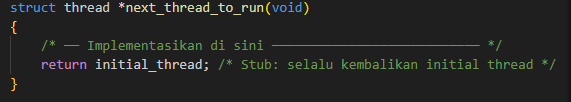
\includegraphics[width=0.85\textwidth]{Figure/12/2.png}
		      \caption{Implementasi fungsi \texttt{next\_thread\_to\_run()} untuk Priority Scheduling.}
		      \label{fig:m12-sesi2}
	      \end{figure}

	      Penjelasan setiap tahap:
	      \begin{itemize}
		      \item \textbf{Tahap 1 (Pemindaian):} Loop menelusuri seluruh isi antrean mulai dari \texttt{ready\_head}. Untuk setiap elemen, bandingkan \texttt{priority}-nya dengan \texttt{best\_prio}. Jika lebih tinggi, catat indeks aktualnya di \texttt{best\_idx} dan perbarui \texttt{best\_prio}. Setelah loop selesai, \texttt{best\_idx} menunjuk ke posisi thread dengan prioritas tertinggi.

		      \item \textbf{Tahap 2 (Pengambilan):} Simpan pointer thread terpilih dari \texttt{ready\_queue[best\_idx]} ke variabel \texttt{next}.

		      \item \textbf{Tahap 3 (Penggeseran):} Karena thread yang diambil mungkin bukan dari posisi depan antrean (berbeda dengan FIFO), elemen-elemen setelahnya harus digeser maju satu posisi untuk menutup celah. Ini dilakukan oleh loop \texttt{while} yang bergerak dari \texttt{best\_idx} hingga \texttt{ready\_tail}. Terakhir, mundurkan \texttt{ready\_tail} dan kurangi \texttt{ready\_count}.
	      \end{itemize}

	      \textit{Catatan penting: Jika muncul error \texttt{implicit declaration of function} saat kompilasi, pastikan Anda tidak menghapus baris \texttt{\#include "thread.h"} dan \texttt{\#include "types.h"} di awal file.}

	      \textit{Jika muncul warning \texttt{comparison of unsigned expression < 0 is always true}, pastikan tipe data \texttt{ready\_count} adalah \texttt{uint32\_t} (bukan \texttt{int}). Cek deklarasi variabel di bagian atas file \texttt{thread.c}.}

	\item \textbf{Simpan} file \texttt{thread.c}. Saat ini \textit{scheduler} Anda sudah berubah dari \textit{Round-Robin} menjadi \textit{Priority Scheduling}.
\end{enumerate}

% -----------------------------------------------------------------
\subsection{Sesi 3: Kompilasi dan Verifikasi Sistem OS}
\label{sec:m12-sesi-3}

Setelah kode \textit{Priority Scheduling} selesai ditulis, kita bisa mengompilasi dan menjalankan sistem untuk melihat hasilnya. Pada sesi ini, kita akan membandingkan keluaran QEMU sebelum dan sesudah modifikasi.

\begin{enumerate}
	\item Lakukan kompilasi sistem operasi Anda dengan \textit{flag} \texttt{PRIORITY\_SCHEDULING}.
	      \begin{lstlisting}[language=bash, caption={Kompilasi dan jalankan dengan Priority Scheduling}]
# Pastikan telah menjalankan make clean sebelumnya
make DEMO=-DPRIORITY_SCHEDULING
make run
    \end{lstlisting}

	      \textit{Jika muncul error \texttt{linker error: undefined reference to `next\_thread\_to\_run'}, berarti ada kesalahan sintaks pada fungsi Anda (misalnya kurung kurawal tidak tertutup). Periksa kembali kode pada Sesi 2.}

	      \textit{Jika kompilasi berhasil tetapi QEMU langsung menampilkan \texttt{KERNEL PANIC}, kemungkinan \texttt{next\_thread\_to\_run()} mengembalikan \texttt{NULL}. Pastikan blok \texttt{if (ready\_count == 0) return initial\_thread;} masih ada di awal fungsi.}

	\item \textbf{Verifikasi Hasil:} Amati keluaran (\textit{output}) di layar QEMU. Bandingkan dengan perilaku sebelum modifikasi.
	      \begin{itemize}
		      \item \textbf{Sebelumnya (Modul 11):} Ketiga \textit{thread} bergantian secara merata tanpa memperhatikan prioritas (\textit{Round-Robin}).
		      \item \textbf{Sekarang (Modul 12):} Thread \texttt{High} (prioritas 50) mendominasi CPU selama 5 tick penuh. Setelah \texttt{High} \textit{exit}, \texttt{Med} (prioritas 31) mendominasi CPU sepenuhnya, sementara \texttt{Low} (prioritas 10) \textbf{tidak pernah mendapat giliran} (\textit{starvation}).
	      \end{itemize}

	      \begin{lstlisting}[caption={Ekspektasi keluaran QEMU setelah Priority Scheduling}]
===================================
  IF-OS  |  Praktikum Sistem Operasi
===================================

Inisialisasi sistem thread...
Demo Minggu 6: Priority Scheduling
(Jika masih Round-Robin, next_thread_to_run() belum dimodifikasi)
(High=50 jalan 5 tick lalu exit, Med=31 mengambil alih, Low=10 terakhir)

[High] tick 0
[High] tick 1
[High] tick 2
[High] tick 3
[High] tick 4
[High] selesai (5 tick)
[Med] tick 0
[Med] tick 1
[Med] tick 2
[Med] tick 3
...            <- Med berjalan terus, Low tidak pernah muncul
    \end{lstlisting}

	      Meskipun \textit{thread} \texttt{Low} memanggil \texttt{yield()} dan masuk kembali ke antrean, \textit{scheduler} selalu memilih \textit{thread} berprioritas tertinggi. Karena \texttt{Med} (31) selalu memiliki prioritas lebih tinggi daripada \texttt{Low} (10), \texttt{Med} akan terus dipilih dan \texttt{Low} \textbf{tidak pernah mendapat giliran sama sekali}.

	      Fenomena ini adalah contoh nyata dari \textbf{\textit{starvation}} yang telah dibahas pada Dasar Teori. Pada skenario ini, \texttt{High} tidak menyebabkan \textit{starvation} permanen karena memiliki batas \texttt{max\_ticks = 5}, tetapi \texttt{Med} (yang berjalan tanpa batas) secara efektif membuat \texttt{Low} kelaparan selamanya. Untuk mengatasi ini, diperlukan mekanisme \textit{aging} sebagaimana dijelaskan pada Dasar Teori, namun implementasinya berada di luar cakupan modul ini.

	\item Ambil tangkapan layar (\textit{screenshot}) hasil eksekusi untuk membuktikan bahwa implementasi \textit{Priority Scheduling} telah berjalan sesuai ekspektasi.
\end{enumerate}

\begin{figure}[htbp]
	\centering
	% TODO: tambahkan screenshot hasil QEMU Priority Scheduling ke Figure/12/1.png
	
\includegraphics[width=0.85\textwidth]{Figure/12/1.png}
	\caption{Keluaran (\textit{output}) QEMU setelah implementasi Priority Scheduling. Thread High (prioritas 50) dieksekusi pertama kali selama 5 tick penuh, kemudian Med (prioritas 31) mendominasi CPU sepenuhnya sementara Low (prioritas 10) mengalami \textit{starvation}.}
	\label{fig:m12-sesi3}
\end{figure}

% ----------------------------------------------------------------
\section{Latihan}

\subsection{Tujuan}

Kerjakan tugas-tugas berikut secara berurutan mengikuti alur sesi pada Modul 11 dan Modul 12. Sertakan bukti berupa tangkapan layar (\textit{screenshot}) QEMU atau penggalan kode yang relevan pada setiap langkah yang diminta.

% ============================================================
\subsection{Sesi 1: Mengamati Perilaku Round-Robin}
% ============================================================

\subsubsection{Persiapan dan Kompilasi}

Pastikan implementasi Minggu 4 sudah berfungsi, lalu kompilasi dengan \textit{flag} \texttt{PRIORITY\_SCHEDULING} diaktifkan.

\begin{enumerate}

	\item Pastikan Anda sudah berada di dalam lingkungan Docker (jalankan \texttt{./run-docker.sh} jika belum) sebelum menjalankan perintah berikut.

	\item Jalankan perintah berikut untuk mengompilasi dan menjalankan kernel:
	      \begin{lstlisting}[language=bash, caption={Compile dan jalankan demo Priority Scheduling}]
make clean
make DEMO=-DPRIORITY_SCHEDULING
make run
    \end{lstlisting}

	      Amati keluaran (\textit{output}) yang muncul selama $\pm$15 detik, lalu ambil tangkapan layar (\textit{screenshot}) pada layar QEMU. Tempel hasil tangkapan layar di sini:


	\item Perhatikan tiga thread yang dibuat di \texttt{kernel.c} dan isilah tabel berikut berdasarkan kode sumber.

	      \begin{table}[htbp]
		      \centering
		      \caption{Konfigurasi thread pada mode \texttt{PRIORITY\_SCHEDULING}}
		      \begin{tabulary}{\textwidth}{|l|c|l|c|}
			      \hline
			      \textbf{Nama} & \textbf{Prioritas} & \textbf{Warna VGA} & \textbf{max\_ticks} \\ \hline
			      Low  & 10 & \textit{[Isi]} & \textit{[Isi]} \\ \hline
			      Med  & \textit{[Isi]} & \textit{[Isi]} & \textit{[Isi]} \\ \hline
			      High & \textit{[Isi]} & \textit{[Isi]} & \textit{[Isi]} \\ \hline
		      \end{tabulary}
	      \end{table}

\end{enumerate}

% ────────────────────────────────────────────────────────────
\subsubsection{Analisis Perilaku Round-Robin}

\begin{enumerate}

	\item Perhatikan urutan keluaran thread di layar QEMU. Isilah tabel berikut untuk mengidentifikasi pola urutan eksekusi.

	      \begin{table}[htbp]
		      \centering
		      \caption{Urutan eksekusi thread yang diamati pada Round-Robin}
		      \begin{tabulary}{\textwidth}{|c|l|c|L|}
			      \hline
			      \textbf{Giliran} & \textbf{Thread} & \textbf{Prioritas} & \textbf{Mengapa dipilih?} \\ \hline
			      1 & \textit{[Isi]} & \textit{[Isi]} & \textit{[Isi: karena masuk antrian pertama]} \\ \hline
			      2 & \textit{[Isi]} & \textit{[Isi]} & \textit{[Isi]} \\ \hline
			      3 & \textit{[Isi]} & \textit{[Isi]} & \textit{[Isi]} \\ \hline
			      4 & \textit{[Isi]} & \textit{[Isi]} & \textit{[Isi: kembali ke depan (FIFO berputar)]} \\ \hline
		      \end{tabulary}
	      \end{table}

	\item Apakah thread \texttt{High} (prioritas 50) mendapat perlakuan istimewa dari \textit{scheduler}? Jelaskan mengapa atau mengapa tidak, berdasarkan kode \texttt{next\_thread\_to\_run()} versi Round-Robin.

	\item Setelah \texttt{High} selesai (tick ke-5), apa yang terjadi pada urutan eksekusi antara \texttt{Low} dan \texttt{Med}? Apakah keduanya tetap bergantian secara adil?

\end{enumerate}

% ============================================================
\subsection{Sesi 2: Implementasi Priority Scheduling}
% ============================================================

\subsubsection{Analisis Kode yang Akan Dirombak}

\begin{enumerate}

	\item Buka file \texttt{src/thread.c} dan perhatikan fungsi \texttt{next\_thread\_to\_run()} versi FIFO. Identifikasi baris kode mana yang menyebabkan scheduler mengabaikan prioritas.

	      \begin{table}[htbp]
		      \centering
		      \caption{Identifikasi kelemahan kode Round-Robin}
		      \begin{tabulary}{\textwidth}{|L|L|}
			      \hline
			      \textbf{Pertanyaan} & \textbf{Jawaban} \\ \hline
			      Baris kode mana yang mengambil thread dari antrian?
			      & \textit{[Isi: tuliskan baris kode tersebut]} \\ \hline
			      Apakah baris tersebut memeriksa field \texttt{priority}?
			      & \textit{[Isi]} \\ \hline
			      Apa yang menentukan urutan pemilihan thread?
			      & \textit{[Isi: urutan masuk antrian / nilai prioritas / ...]} \\ \hline
		      \end{tabulary}
	      \end{table}

\end{enumerate}

% ────────────────────────────────────────────────────────────
\subsubsection{Implementasi \texttt{next\_thread\_to\_run()} (Priority)}

\begin{enumerate}

	\item Salin kode \texttt{next\_thread\_to\_run()} versi Priority Scheduling yang telah Anda tulis:

	      \begin{lstlisting}[language=C, caption={Implementasi \texttt{next\_thread\_to\_run()} versi Priority oleh mahasiswa}]
struct thread *next_thread_to_run(void) {

    /* Tulis implementasi Anda di sini */

}
    \end{lstlisting}

	\item Jelaskan secara singkat logika tiga tahap pada implementasi Anda:
	      \begin{enumerate}
		      \item[(a)] Tahap 1 (Pemindaian): Bagaimana Anda menelusuri isi antrian untuk mencari thread dengan prioritas tertinggi?

		      \item[(b)] Tahap 2 (Pengambilan): Mengapa Anda perlu menyimpan pointer ke thread terpilih sebelum melakukan penggeseran?

		      \item[(c)] Tahap 3 (Penggeseran): Mengapa perlu menggeser elemen setelah posisi terpilih? Apa yang terjadi jika langkah ini dilewati?
	      \end{enumerate}

	\item Jika dua thread memiliki prioritas yang sama (misalnya keduanya \texttt{PRI\_DEFAULT}), thread mana yang akan dipilih oleh implementasi Anda? Apakah ini perilaku yang diinginkan? (Kaitkan jawaban Anda dengan hasil eksperimen pada Eksplorasi 2)

\end{enumerate}

% ============================================================
\subsection{Sesi 3: Kompilasi dan Verifikasi}
% ============================================================

\begin{enumerate}

	\item \textit{Compile} ulang dan jalankan kernel setelah implementasi Priority Scheduling:
	      \begin{lstlisting}[language=bash, caption={Compile dan jalankan dengan Priority Scheduling}]
make clean
make DEMO=-DPRIORITY_SCHEDULING
make run
    \end{lstlisting}

	      Sertakan tangkapan layar (\textit{screenshot}) keluaran (\textit{output}) QEMU \textbf{sebelum} dan \textbf{sesudah} modifikasi scheduler secara berdampingan.


	\item Verifikasi urutan keluaran (\textit{output}) yang benar. Isilah tabel berikut berdasarkan pengamatan Anda.

	      \begin{table}[htbp]
		      \centering
		      \caption{Perbandingan urutan eksekusi sebelum dan sesudah modifikasi}
		      \begin{tabulary}{\textwidth}{|c|L|L|}
			      \hline
			      \textbf{Giliran ke-} & \textbf{Round-Robin (Modul 11)} & \textbf{Priority Scheduling (Modul 12)} \\ \hline
			      1 & \textit{[Isi: Low / Med / High?]} & \textit{[Isi]} \\ \hline
			      2 & \textit{[Isi]} & \textit{[Isi]} \\ \hline
			      3 & \textit{[Isi]} & \textit{[Isi]} \\ \hline
			      4 & \textit{[Isi]} & \textit{[Isi]} \\ \hline
			      6 (setelah High exit) & \textit{[Isi]} & \textit{[Isi]} \\ \hline
		      \end{tabulary}
	      \end{table}

	\item Apakah thread \texttt{Low} (prioritas 10) mendapat giliran setelah thread \texttt{High} selesai? Jelaskan mengapa hal tersebut terjadi (kaitkan dengan mekanisme pemindaian antrian pada skenario ini).

	\item Isilah tabel ringkasan perbandingan kedua algoritma berdasarkan hasil praktikum yang telah dilakukan.

	      \begin{table}[htbp]
		      \centering
		      \caption{Ringkasan perbandingan Round-Robin vs Priority Scheduling}
		      \begin{tabulary}{\textwidth}{|l|L|L|}
			      \hline
			      \textbf{Aspek} & \textbf{Round-Robin} & \textbf{Priority Scheduling} \\ \hline
			      Prinsip pemilihan
			      & \textit{[Isi]} & \textit{[Isi]} \\ \hline
			      Fairness
			      & \textit{[Isi]} & \textit{[Isi]} \\ \hline
			      Apakah High didahulukan?
			      & \textit{[Isi]} & \textit{[Isi]} \\ \hline
			      Risiko utama
			      & \textit{[Isi]} & \textit{[Isi]} \\ \hline
		      \end{tabulary}
	      \end{table}

\end{enumerate}

% ============================================================
\subsection{Eksplorasi Mandiri}
% ============================================================

\begin{enumerate}

	% ── Eksplorasi 1 ─────────────────────────────────────────
	\item \textbf{Eksperimen mengubah nilai prioritas.}\\
	      Pada \texttt{kernel.c}, tukar nilai prioritas thread \texttt{Low} dan \texttt{High} sehingga \texttt{Low} mendapat prioritas 50 dan \texttt{High} mendapat prioritas 10. \textit{Compile} ulang dan jalankan.

	      \begin{lstlisting}[language=bash, caption={Kompilasi untuk eksperimen tukar prioritas}]
make clean && make DEMO=-DPRIORITY_SCHEDULING && make run
    \end{lstlisting}

	      \begin{enumerate}
		      \item[(a)] Sertakan tangkapan layar (\textit{screenshot}) hasil QEMU.


		      \item[(b)] Thread mana yang sekarang dieksekusi terlebih dahulu? Apakah hasilnya sesuai dengan ekspektasi?
	      \end{enumerate}

	      % Eksplorasi 2 
	\item \textbf{Simulasi Round-Robin dengan Prioritas.}\\
	      Ubah parameter prioritas pada ketiga \textit{thread} di \texttt{kernel.c} agar semuanya memiliki prioritas yang \textbf{sama persis} (misalnya ketiganya diberi \texttt{PRI\_DEFAULT} atau 31). Pastikan \texttt{max\_ticks} untuk \texttt{High} tetap 5. \textit{Compile} ulang dan jalankan.

	      \begin{enumerate}
		      \item[(a)] Sertakan tangkapan layar (\textit{screenshot}) hasil QEMU.


		      \item[(b)] Bagaimana perilaku \textit{scheduler} saat semua antrian memiliki nilai prioritas yang setara? Apakah kembali bertindak seperti \textit{Round-Robin} (FIFO)? Jelaskan alasannya berdasarkan implementasi kode Anda.
	      \end{enumerate}

	      % ── Eksplorasi 3 ─────────────────────────────────────────
	\item \textbf{Refleksi: Solusi untuk starvation.}\\
	      Berdasarkan konsep \textit{aging} yang telah dipelajari pada dasar teori Modul~12:
	      \begin{enumerate}
		      \item[(a)] Jelaskan bagaimana teknik \textit{aging} dapat mengatasi \textit{starvation} yang Anda amati pada eksperimen di atas.
		      \item[(b)] Komponen apa yang perlu ditambahkan pada \texttt{next\_thread\_to\_run()} agar \textit{aging} dapat bekerja? Jelaskan secara konseptual (tidak perlu menulis kode).
	      \end{enumerate}

\end{enumerate}


%%%%%%%%%%%%%%%%%%%%% KONTRIBUSI PENULIS %%%%%%%%%%%%%%%%%%%%%
\cleardoublepage
\section*{Kontribusi Penulis}
\addcontentsline{toc}{section}{Kontribusi Penulis}

Bagian ini mencantumkan kontribusi masing-masing individu dalam penyusunan buku ajar ini.

\subsection*{Penulis}
\begin{itemize}[label=]
	\item Ahmat Prayoga Sembiring
	\item Andryano Shevchenko Limbong
	\item Aziz Kurniawan
	\item Dito Rifki Irawan
	\item Ebentua Philippus Limbong
	\item Elsa Elisa Yohana Sianturi
	\item Fathan Andi Kartagama
	\item Miftahul Khoiriyah
	\item Muhammad Bintang Al-Fasya
	\item Muhammad Fadhil Zurani
	\item Reza Chairul Manam
	\item Stevanus Cahya Anggara
	\item Varasina Farmadani
	\item Zakhi Algifari
\end{itemize}

\subsection*{Editor dan Proofreader}
\begin{itemize}[label=]
	\item Eko Dwi Nugroho
	\item I Wayan Wiprayoga Wisesa
	\item Ilham Firman Ashari
	\item Martin Clinton Tosima Manullang
\end{itemize}


%%%%%%%%%%%%%%%%%%%%% REFERENSI %%%%%%%%%%%%%%%%%%%%%
\renewcommand{\bibname}{Bibliography}
\cleardoublepage
\addcontentsline{toc}{chapter}{Bibliography}
\bibliographystyle{IEEEtran}
\bibliography{Referensi}

% ===== HALAMAN BELAKANG =====
\cleardoublepage
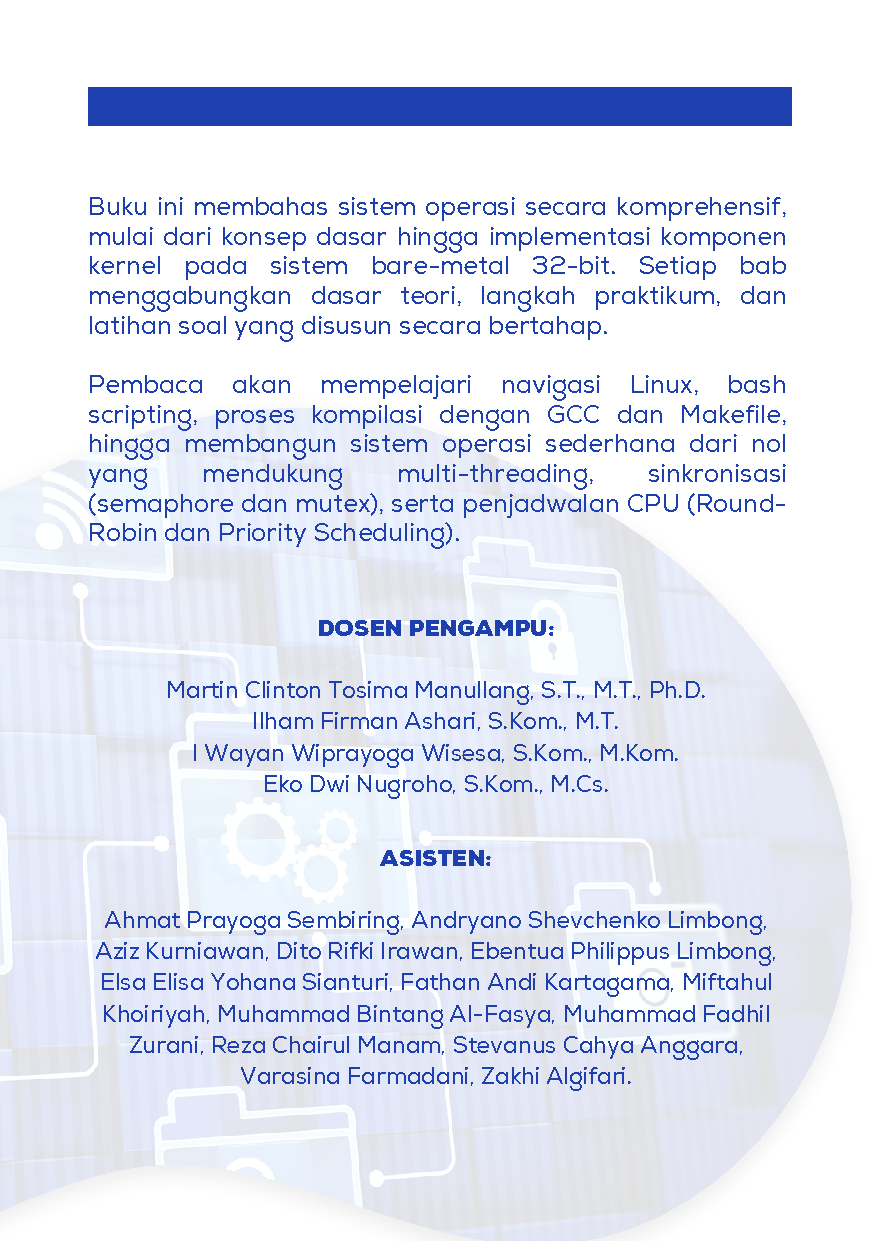
\includepdf[pages=1,noautoscale]{Figure/cover-back.pdf}

\end{document}
